\documentclass[11pt]{article}

% Load essential packages
\usepackage[utf8]{inputenc}
\usepackage[T1]{fontenc}
\usepackage{amsmath,amssymb,amsthm}
\usepackage{graphicx}
\usepackage[numbers]{natbib}
\usepackage[colorlinks,citecolor=blue,urlcolor=blue]{hyperref}
\usepackage{booktabs}
\usepackage{multirow}
\usepackage{algorithm}
\usepackage{algorithmic}
\usepackage{cleveref}

% Page layout for standard academic paper
\usepackage[letterpaper,margin=1in]{geometry}
\usepackage{setspace}
\onehalfspacing

% Math settings
\allowdisplaybreaks
\numberwithin{equation}{section}

% Theorem environments
\theoremstyle{plain}
\newtheorem{theorem}{Theorem}[section]
\newtheorem{lemma}[theorem]{Lemma}
\newtheorem{proposition}[theorem]{Proposition}
\newtheorem{corollary}[theorem]{Corollary}

\theoremstyle{definition}
\newtheorem{definition}[theorem]{Definition}
\newtheorem{remark}[theorem]{Remark}
\newtheorem{example}[theorem]{Example}

% Custom commands
\newcommand{\R}{\mathbb{R}}
\newcommand{\N}{\mathbb{N}}
\newcommand{\E}{\mathbb{E}}
\newcommand{\Var}{\text{Var}}
\newcommand{\Cov}{\text{Cov}}
\newcommand{\given}{\,|\,}

\begin{document}

\title{Copula-Extended Max-and-Smooth for Latent Gaussian Models With Data-Level Dependence}

\author{Your Name\thanks{Department of Statistics, Your Institution. Email: your.email@institution.edu} \and
Co-author Name\thanks{Department of Statistics, Co-author Institution. Email: coauthor.email@institution.edu}}

\date{\today}

\maketitle

\begin{abstract}
Abstract text goes here.
\end{abstract}

\section{Introduction}
% Introduction content



\section{Latent Gaussian Models}
\label{sec:lgm}
% Latent Gaussian Models

\subsection{Model Structure} \label{subsubsec:model-structure}
Latent Gaussian models constitute a class of Bayesian hierarchical models characterized by a three-level structure:

\begin{enumerate}
    \item \textbf{Data level}: The observations $\mathbf{y} = (y_1, \ldots, y_n)^T$ are modeled conditionally on latent parameters $\boldsymbol{\eta}$ and hyperparameters $\boldsymbol{\theta}$, with density $\pi(\mathbf{y}|\boldsymbol{\eta}, \boldsymbol{\theta})$.

    \item \textbf{Latent level}: The latent parameters $\boldsymbol{\eta}$ follow a Gaussian distribution conditional on hyperparameters $\boldsymbol{\theta}$:
    \begin{equation}
        \pi(\boldsymbol{\eta}|\boldsymbol{\theta}) = \mathcal{N}(\boldsymbol{\eta}|\boldsymbol{\mu}(\boldsymbol{\theta}), \mathbf{\Sigma}(\boldsymbol{\theta})).
    \end{equation}

    \item \textbf{Hyperparameter level}: The hyperparameters $\boldsymbol{\theta}$ are assigned a prior density $\pi(\boldsymbol{\theta})$.
\end{enumerate}

The defining characteristic of LGMs is the Gaussian prior on the latent field $\boldsymbol{\eta}$. For computational efficiency, the latent field is often structured as a Gaussian Markov Random Field (GMRF) with a sparse precision matrix $\mathbf{Q}_{\boldsymbol{\eta}}(\boldsymbol{\theta}) = \mathbf{\Sigma}^{-1}(\boldsymbol{\theta})$, facilitating efficient inference even in high dimensions.

In standard LGMs, as described by \cite{rue2009approximate}, a univariate link function connects a parameter of interest at the data level to a structured additive predictor at the latent level:

\begin{equation}
    g(\mu_i) = \eta_i,
\end{equation}

where $\mu_i = \mathrm{E}(y_i|\eta_i, \boldsymbol{\theta})$ or $\mu_i = Q_p(y_i|\eta_i, \boldsymbol{\theta})$ for some quantile function $Q_p$, and $g(\cdot)$ is the link function. The structured additive predictor $\eta_i$ typically takes the form:

\begin{equation}
    \eta_i = \beta_0 + \sum_{k=1}^K \beta_k z_{i,k} + \sum_{j=1}^J u_j a_{i,j} + \epsilon_i,
\end{equation}

where $\beta_0$ is an intercept, $\{\beta_k\}$ are linear fixed effects, $\{u_j\}$ are random effects with specified dependency structures, and $\{\epsilon_i\}$ are unstructured model errors.

\subsubsection{Extended LGMs with Multivariate Link Functions} \label{subsubsec:ext-lgm}
Many applications require modeling multiple parameters of the data distribution simultaneously, motivating the development of extended LGMs with multivariate link functions \citep{geirsson2020lgm}. In these models, multiple parameters of the data distribution are linked to separate latent Gaussian fields, providing greater flexibility in capturing complex data structures.

For extended LGMs, we assume that the data can be grouped according to some structure (e.g., spatial locations, time points, or categories), with each group $i$ having $n_i$ observations. Let the total number of groups be $G$. For group $i$, the parameters are denoted by $\boldsymbol{\psi}_i = (\psi_{1,i}, \psi_{2,i}, \ldots, \psi_{M,i})^T \in D$, where $D$ is a subspace of $\mathbb{R}^M$ and $M$ is the number of parameters. The joint density for all observations is:

\begin{equation}
    \pi(\mathbf{y}|\boldsymbol{\psi}_1, \boldsymbol{\psi}_2, \ldots, \boldsymbol{\psi}_G) = \prod_{i=1}^G \pi(\mathbf{y}_i|\boldsymbol{\psi}_i) = \prod_{i=1}^G \prod_{j \in A_i} \pi(y_{i,j}|\boldsymbol{\psi}_i),
\end{equation}

where $A_i$ is the index set for group $i$.

We define an $M$-variate link function $\mathbf{g}: D \rightarrow \mathbb{R}^M$ such that:

\begin{equation}
    \mathbf{g}(\boldsymbol{\psi}_i) = (\eta_{1,i}, \eta_{2,i}, \ldots, \eta_{M,i})^T = \boldsymbol{\eta}_i \in \mathbb{R}^M.
\end{equation}

For each parameter type $m \in \{1, \ldots, M\}$, we specify a linear model for the latent parameters $\boldsymbol{\eta}_m = (\eta_{m,1}, \ldots, \eta_{m,G})^T$:

\begin{equation}
    \boldsymbol{\eta}_m = \mathbf{X}_m \boldsymbol{\beta}_m + \mathbf{A}_m \mathbf{u}_m + \boldsymbol{\epsilon}_m,
\end{equation}

where $\boldsymbol{\beta}_m$ represents fixed effects, $\mathbf{X}_m$ is the corresponding design matrix, $\mathbf{u}_m$ represents random effects, $\mathbf{A}_m$ is the corresponding weight matrix, and $\boldsymbol{\epsilon}_m$ represents unstructured error terms. The terms $\boldsymbol{\beta}_m$, $\mathbf{u}_m$, and $\boldsymbol{\epsilon}_m$ are assigned Gaussian prior densities and are assumed to be a priori independent.


\section{Max-and-Smooth}
\label{sec:maxsmooth}
% Max & Smooth: A Two-Step Inference Approach

\subsection{Overview and Motivation} \label{subsec:ms-overview}
Max \& Smooth \citep{hrafnkelsson2021max} is a two-step approximate Bayesian inference method designed for extended LGMs with independent data replicates. It addresses the limitations of existing methods by providing an efficient and accurate inference scheme for models with multivariate link functions and high-dimensional latent fields.

The key insight of Max \& Smooth is to approximate the likelihood function with a Gaussian density, which, when combined with the Gaussian prior for the latent field, results in a computationally tractable Gaussian-Gaussian model. This approach allows for fast and accurate Bayesian inference while properly propagating uncertainty from the data to the posterior distributions.

Max \& Smooth is particularly well-suited for datasets with independent replicates, where the Gaussian approximation to the likelihood becomes increasingly accurate as the number of replicates grows, following the asymptotic behavior of likelihood functions \citep{schervish1995theory}.

\subsection{Step 1: Gaussian Approximation of the Likelihood (Max)} \label{subsec:ms-step1}
The first step of Max \& Smooth involves approximating the likelihood function with a Gaussian density. This approximation is performed for each group of independent data replicates separately, leveraging the conditional independence assumption.

Let $L(\boldsymbol{\eta}|\mathbf{y})$ denote the likelihood function. We consider two different Gaussian approximations:

\begin{enumerate}
    \item \textbf{First Gaussian approximation} (based on the maximum likelihood estimate and observed information):
    \begin{equation}
        \hat{L}(\boldsymbol{\eta}|\mathbf{y}) = N(\boldsymbol{\eta}|\hat{\boldsymbol{\eta}}, \mathbf{\Sigma}_{\boldsymbol{\eta}\mathbf{y}})
    \end{equation}
    where $\hat{\boldsymbol{\eta}}$ is the maximum likelihood estimate of $\boldsymbol{\eta}$, and $\mathbf{\Sigma}_{\boldsymbol{\eta}\mathbf{y}} = (\mathbf{I}_{\boldsymbol{\eta}\mathbf{y}})^{-1}$, with $\mathbf{I}_{\boldsymbol{\eta}\mathbf{y}}$ being the observed information matrix evaluated at $\hat{\boldsymbol{\eta}}$.

    \item \textbf{Second Gaussian approximation} (based on the mean and covariance of the normalized likelihood):
    \begin{equation}
        \tilde{L}(\boldsymbol{\eta}|\mathbf{y}) = N(\boldsymbol{\eta}|\tilde{\boldsymbol{\eta}}, \boldsymbol{\Omega}_{\boldsymbol{\eta}\mathbf{y}})
    \end{equation}
    where $\tilde{\boldsymbol{\eta}}$ and $\boldsymbol{\Omega}_{\boldsymbol{\eta}\mathbf{y}}$ are the mean and covariance matrix of the normalized likelihood function, respectively.
\end{enumerate}

For each group $i$, the likelihood contribution $L(\boldsymbol{\eta}_i|\mathbf{y}_i)$ is approximated independently. The approximated likelihood for the entire model is then:

\begin{equation}
    \hat{L}(\boldsymbol{\eta}|\mathbf{y}) = \prod_{i=1}^G \hat{L}(\boldsymbol{\eta}_i|\mathbf{y}_i) = N(\boldsymbol{\eta}|\hat{\boldsymbol{\eta}}, \mathbf{Q}_{\boldsymbol{\eta}\mathbf{y}}^{-1}),
\end{equation}

where $\mathbf{Q}_{\boldsymbol{\eta}\mathbf{y}} = \mathbf{\Sigma}_{\boldsymbol{\eta}\mathbf{y}}^{-1}$ is a block-diagonal precision matrix, with blocks corresponding to the inverse observed information matrices for each group.

\subsection{Step 2: Bayesian Inference with the Gaussian-Gaussian Model (Smooth)} \label{subsec:ms-step2}
In the second step of Max \& Smooth, we treat the estimates from the first step ($\hat{\boldsymbol{\eta}}$ or $\tilde{\boldsymbol{\eta}}$) as noisy measurements of the latent field, with known noise covariance matrices ($\mathbf{\Sigma}_{\boldsymbol{\eta}\mathbf{y}}$ or $\boldsymbol{\Omega}_{\boldsymbol{\eta}\mathbf{y}}$). This leads to a Gaussian-Gaussian pseudo model, which we can write hierarchically as:

\begin{align}
    \pi(\hat{\boldsymbol{\eta}}|\boldsymbol{\eta}, \mathbf{Q}_{\boldsymbol{\eta}\mathbf{y}}, \boldsymbol{\theta}) &= N(\hat{\boldsymbol{\eta}}|\boldsymbol{\eta}, \mathbf{Q}_{\boldsymbol{\eta}\mathbf{y}}^{-1}) \\
    \pi(\boldsymbol{\eta}|\boldsymbol{\nu}, \boldsymbol{\theta}) &= N(\boldsymbol{\eta}|\mathbf{Z}\boldsymbol{\nu}, \mathbf{Q}_{\boldsymbol{\epsilon}}^{-1}) \\
    \pi(\boldsymbol{\nu}|\boldsymbol{\theta}) &= N(\boldsymbol{\nu}|\boldsymbol{\mu}_{\boldsymbol{\nu}}, \mathbf{Q}_{\boldsymbol{\nu}}^{-1})
\end{align}

where $\boldsymbol{\nu}$ contains all the latent parameters that are assigned a Gaussian prior, and $\mathbf{Z}$ is a matrix that relates $\boldsymbol{\eta}$ to $\boldsymbol{\nu}$.

The approximate posterior distribution can be written as:

\begin{equation}
    \hat{\pi}(\boldsymbol{\eta}, \boldsymbol{\nu}, \boldsymbol{\theta}|\mathbf{y}) \propto \pi(\boldsymbol{\theta}) \pi(\boldsymbol{\eta}, \boldsymbol{\nu}|\boldsymbol{\theta}) \hat{L}(\boldsymbol{\eta}|\mathbf{y}).
\end{equation}

\subsection{Implementation and Computational Considerations} \label{subsec:ms-implementation}
The Max \& Smooth approach offers significant computational advantages for high-dimensional LGMs with independent data replicates:

\begin{enumerate}
    \item \textbf{Parallel computation}: The first step (Max) can be parallelized across groups, as the likelihood approximation for each group is performed independently.

    \item \textbf{Sparse matrix operations}: When the precision matrices at the latent level are sparse (as is typical with GMRFs), sparse matrix algorithms can be employed for efficient computation in the second step (Smooth).

    \item \textbf{Scalability with replicates}: The computational cost of the second step is insensitive to the number of data replicates, making Max \& Smooth particularly efficient for datasets with many replicates.
\end{enumerate}

\subsection{Limitations and Future Directions} \label{subsec:limitations}
While Max \& Smooth provides an efficient inference framework for extended LGMs, it has several limitations that motivate further methodological developments:

\begin{enumerate}
    \item \textbf{Independent replicates}: The method is designed for datasets with independent replicates. For data with complex dependence structures at the observation level, the current formulation may not be directly applicable.

    \item \textbf{Data-level dependence}: Max \& Smooth, like standard LGMs, focuses on modeling dependence at the parameter level through the latent Gaussian field. However, many applications require modeling dependence at the data level, especially when the data exhibit complex dependency patterns that cannot be fully captured by parameter-level modeling alone.

    \item \textbf{Approximation accuracy}: The accuracy of the Gaussian approximation to the likelihood depends on the number of data replicates and the specific form of the data distribution. With a small number of replicates or heavily skewed distributions, the approximation may be less accurate.
\end{enumerate} 

\section{A Spatial Gaussian Copula}
\label{sec:copulas}
% Chapter 3: Copulas and the Matérn Spatial Copula


While Latent Gaussian Models (LGMs) provide a powerful framework for capturing parameter-level dependencies, they have limitations in modeling complex dependence structures at the data level. In Chapter 3, we introduced the Max \& Smooth approach for approximate Bayesian inference in LGMs, which efficiently handles parameter-level dependence. This chapter addresses the complementary challenge of modeling dependence at the data level through copulas, with a particular focus on spatial applications.

\subsection{Essential Background}

Copulas provide a mathematical framework for separating the dependence structure of a multivariate distribution from its marginal distributions. The cornerstone of copula theory is Sklar's theorem, which states that any multivariate distribution function $F$ with marginals $F_1,\ldots,F_d$ can be expressed as:

\begin{equation}
F(x_1,\ldots,x_d) = C(F_1(x_1),\ldots,F_d(x_d))
\end{equation}

where $C$ is a copula function. If the marginals are continuous, this copula is unique.

The joint density function $f$ of a multivariate distribution can be expressed in terms of the copula density $c$ and the marginal densities $f_i$ as:

\begin{equation}
f(x_1,\ldots,x_d) = c(F_1(x_1),\ldots,F_d(x_d)) \prod_{i=1}^d f_i(x_i)
\end{equation}

This decomposition enables two-stage inference procedures where marginal distributions and dependence structure can be modeled separately, providing significant modeling flexibility.

\subsection{Gaussian Copulas}
The Gaussian copula is of particular interest for spatial modeling due to its connection with multivariate normal distributions and its analytical tractability. For a correlation matrix $\mathbf{R}$, the Gaussian copula is defined as:

\begin{equation}
C_{\mathbf{R}}^{\text{Gauss}}(u_1, \ldots, u_d) = \Phi_{\mathbf{R}}(\Phi^{-1}(u_1), \ldots, \Phi^{-1}(u_d))
\end{equation}

where $\Phi_{\mathbf{R}}$ is the joint CDF of a multivariate normal distribution with mean vector 0 and correlation matrix $\mathbf{R}$, and $\Phi^{-1}$ is the quantile function of the standard normal distribution.

The density of the Gaussian copula is:

\begin{equation}
c_{\mathbf{R}}^{\text{Gauss}}(u_1, \ldots, u_d) = \frac{1}{|\mathbf{R}|^{1/2}} \exp\left(-\frac{1}{2}\mathbf{z}^T(\mathbf{R}^{-1} - \mathbf{I})\mathbf{z}\right)
\end{equation}

where $\mathbf{z} = (\Phi^{-1}(u_1), \ldots, \Phi^{-1}(u_d))^T$ and $\mathbf{I}$ is the identity matrix.

A crucial observation is that the Gaussian copula is completely determined by the correlation matrix $\mathbf{R}$, which, by definition, has unit diagonal entries. This requirement becomes central to our methodological development in the context of precision-based spatial modeling.

\subsection{Spatial Dependence Modeling}

\subsubsection{Challenges in Spatial Copula Modeling}
Spatial datasets present specific challenges for copula-based modeling:

\begin{enumerate}
\item \textbf{High dimensionality}: Spatial datasets often involve hundreds or thousands of locations.
\item \textbf{Spatial consistency}: The dependence structure must respect spatial relationships.
\item \textbf{Computational tractability}: Efficient methods are needed for high-dimensional models.
\end{enumerate}

\subsection{Gaussian Copulas for Spatial Data}
For locations $\mathbf{s}_1, \ldots, \mathbf{s}_n$, a spatial Gaussian process is traditionally constructed by specifying a correlation function $\rho(\mathbf{s}_i, \mathbf{s}_j; \boldsymbol{\theta})$ that depends on the spatial locations and parameter vector $\boldsymbol{\theta}$.

The Matérn correlation function is particularly flexible for spatial modeling:

\begin{equation}
\rho(\mathbf{s}_i, \mathbf{s}_j; \phi, \nu) = \frac{2^{1-\nu}}{\Gamma(\nu)}\left(\sqrt{2\nu}\frac{\|\mathbf{s}_i - \mathbf{s}_j\|}{\phi}\right)^{\nu}K_{\nu}\left(\sqrt{2\nu}\frac{\|\mathbf{s}_i - \mathbf{s}_j\|}{\phi}\right)
\end{equation}

where $K_{\nu}$ is the modified Bessel function of the second kind, $\phi$ is a range parameter, and $\nu$ is a smoothness parameter.

However, constructing and manipulating the correlation matrix $\mathbf{R}$ directly becomes computationally prohibitive for large spatial datasets, motivating precision-based approaches.

\subsection{GMRF-Based Approaches}
Gaussian Markov Random Fields (GMRFs) offer computational advantages for large spatial datasets through sparse precision matrices. For spatial modeling with GMRFs, the precision matrix $\mathbf{Q}$ is typically constructed based on neighborhood relationships, leading to sparse structures that enable efficient computation.

Recent developments have established connections between certain GMRFs and Gaussian fields with Matérn covariance functions through the stochastic partial differential equation (SPDE) approach. This connection allows approximating continuous spatial Gaussian fields using GMRFs, combining the flexibility of Matérn models with the computational efficiency of sparse precision matrices.

However, a fundamental challenge arises when attempting to use GMRF precision structures for Gaussian copula modeling: Gaussian copulas require correlation matrices (matrices with unit diagonal entries), whereas the inverse of precision matrices from GMRFs do not generally have this property. This observation motivates our development of a systematic approach to construct precision matrices that, when inverted, produce valid correlation matrices.

\subsection{The Matérn-like Spatial Copula}

\subsubsection{Definition and Construction}
We introduce a spatial Gaussian copula for data on a regular grid, which combines the flexibility of the Matérn covariance function with the computational efficiency of GMRFs while ensuring that the inverse of the precision matrix yields a correlation matrix.

For locations $\mathbf{s}_1, \ldots, \mathbf{s}_n$ on a regular grid, we define the precision matrix:

\begin{equation}
\mathbf{Q} = (\mathbf{Q}_{\rho_1} \otimes \mathbf{I} + \mathbf{I} \otimes \mathbf{Q}_{\rho_2})^{\nu+1}
\end{equation}

where $\mathbf{Q}_{\rho_1}$ and $\mathbf{Q}_{\rho_2}$ are precision matrices for one-dimensional AR(1) processes in the $x$ and $y$ directions, respectively, $\otimes$ denotes the Kronecker product, and $\nu$ is a smoothness parameter.

The precision matrix $\mathbf{Q}_{\rho}$ for a one-dimensional AR(1) process with correlation parameter $\rho$ is given by:

\begin{equation}
\mathbf{Q}_{\rho} = \frac{1}{1-\rho^2}
\begin{bmatrix}
1 & -\rho & 0 & \cdots & 0 \\
-\rho & 1+\rho^2 & -\rho & \cdots & 0 \\
0 & -\rho & 1+\rho^2 & \cdots & 0 \\
\vdots & \vdots & \vdots & \ddots & \vdots \\
0 & 0 & 0 & \cdots & 1
\end{bmatrix}
\end{equation}

After computing the diagonal entries of $\mathbf{\Sigma} = \mathbf{Q}^{-1}$, we standardize $\mathbf{Q}$ to obtain $\tilde{\mathbf{Q}} = \mathbf{D}\mathbf{Q}\mathbf{D}$, where $\mathbf{D}$ is a diagonal matrix with entries $D_{ii} = \sqrt{\Sigma_{ii}}$. The Matérn spatial copula is then defined as:

\begin{equation}
C_{\tilde{\mathbf{Q}}}^{\text{Matérn}}(u_1, \ldots, u_n) = \Phi_{\mathbf{R}}(\Phi^{-1}(u_1), \ldots, \Phi^{-1}(u_n))
\end{equation}

where $\mathbf{R} = \tilde{\mathbf{Q}}^{-1}$ is a correlation matrix.

\subsection{Efficient Spectral Computation}
The key computational challenge in working with the Matérn spatial copula is efficiently evaluating the copula density, which requires computing the log-determinant $\log|\mathbf{R}|$ and the quadratic form $\mathbf{z}^T(\mathbf{R}^{-1} - \mathbf{I})\mathbf{z}$ without explicitly forming the potentially massive $n_1 n_2 \times n_1 n_2$ precision matrix $\mathbf{Q}$.

We exploit the spectral structure of $\mathbf{Q}$ to perform these computations efficiently. The eigenvalues and eigenvectors of $\mathbf{Q}$ can be derived from those of the much smaller matrices $\mathbf{Q}_{\rho_1}$ and $\mathbf{Q}_{\rho_2}$. Specifically, if $\mathbf{Q}_{\rho_1} = \mathbf{V}_1 \mathbf{\Lambda}_1 \mathbf{V}_1^T$ and $\mathbf{Q}_{\rho_2} = \mathbf{V}_2 \mathbf{\Lambda}_2 \mathbf{V}_2^T$, then the eigenvalues of $\mathbf{Q}$ are given by $(\lambda_{1,i} + \lambda_{2,j})^{\nu+1}$ for all pairs $(i,j)$, and the corresponding eigenvectors are $\mathbf{v}_{1,i} \otimes \mathbf{v}_{2,j}$.

Rather than constructing $\mathbf{Q}$ explicitly, we iterate over the eigenvalue-eigenvector pairs of the smaller matrices to efficiently compute:

\begin{enumerate}
\item \textbf{Marginal variances} for standardization, by accumulating contributions from each eigenvalue-eigenvector pair:
   \begin{equation}
   \Sigma_{kk} = \sum_{i=1}^{n_1}\sum_{j=1}^{n_2} \frac{(\mathbf{v}_{1,i} \otimes \mathbf{v}_{2,j})_k^2}{(\lambda_{1,i} + \lambda_{2,j})^{\nu+1}}
   \end{equation}

\item \textbf{Log-determinant}, by summing over eigenvalues:
   \begin{align}
   \log|\tilde{\mathbf{Q}}| &= \log|\mathbf{D}\mathbf{Q}\mathbf{D}| = \log|\mathbf{Q}| + 2\sum_{i=1}^n \log D_{ii} \\
   \log|\mathbf{Q}| &= (\nu+1)\sum_{i=1}^{n_1}\sum_{j=1}^{n_2} \log(\lambda_{1,i} + \lambda_{2,j})
   \end{align}

\item \textbf{Quadratic form}, by accumulating projections onto each eigenvector:
   \begin{equation}
   \mathbf{z}^T\tilde{\mathbf{Q}}\mathbf{z} = \sum_{i=1}^{n_1}\sum_{j=1}^{n_2} (\lambda_{1,i} + \lambda_{2,j})^{\nu+1} [(\mathbf{D}\mathbf{z})^T(\mathbf{v}_{1,i} \otimes \mathbf{v}_{2,j})]^2
   \end{equation}
\end{enumerate}

This iterative approach completely avoids forming the full matrix $\mathbf{Q}$ or its inverse, making the computations tractable even for very large spatial grids.

For even larger spatial fields, circulant approximations can further enhance computational efficiency. By approximating $\mathbf{Q}_{\rho_1}$ and $\mathbf{Q}_{\rho_2}$ with circulant matrices, the precision matrix $\mathbf{Q}$ becomes a block circulant matrix with circulant blocks (BCCB). This allows us to use the 2D Fast Fourier Transform (FFT) for efficient computation of the log-determinant and quadratic form, again without ever forming the full precision matrix.

A folded circulant approximation further refines this approach by employing reflected boundary conditions, providing improved accuracy near the edges of the spatial domain while maintaining computational efficiency.

\subsection{Properties and Advantages}
The Matérn spatial copula offers several advantages for spatial modeling:

\begin{enumerate}
\item \textbf{Flexible spatial dependence}: The parameters $\rho_1$, $\rho_2$, and $\nu$ control the range of spatial dependence and the smoothness of the field.

\item \textbf{Computational efficiency}: The precision-based formulation and spectral methods enable efficient computation even for large spatial grids.

\item \textbf{Connection to GMRFs}: The approach establishes a direct link between GMRFs and copula models, leveraging the computational advantages of GMRFs while maintaining the flexibility of copula-based modeling.

\item \textbf{Adaptability}: The framework can accommodate anisotropic dependence structures and can be extended to more complex precision matrices.
\end{enumerate}

This development addresses a fundamental challenge in spatial copula modeling: how to construct precision matrices whose inverses have unit diagonal entries, enabling the use of GMRF structures within the Gaussian copula framework.



\section{Copula-Extended Max-and-Smooth}
\label{sec:extended}
% Chapter 4: Copula-Extended Max-and-Smooth

In Chapters \ref{sec:lgm} and \ref{sec:copulas}, we established the foundations of Latent Gaussian Models (LGMs) with the Max \& Smooth inference approach and introduced the Matérn spatial copula for modeling dependence at the data level.

This chapter presents a novel three-step inference approach that unifies these complementary methodologies, creating a comprehensive framework for modeling dependence at both parameter and data levels. Our approach extends the Max \& Smooth methodology to accommodate data-level dependence through copulas, while maintaining computational efficiency and proper uncertainty propagation. The resulting model---which we refer to as a Copula-Extended Latent Gaussian Model (CELGM)---combines the strengths of both approaches, offering enhanced flexibility for complex spatial and spatio-temporal applications.

The inference procedure is as follows:
\begin{enumerate}
    \item \textbf{Step 1}: Estimate copula parameters from the empirical cumulative distribution function of the data
    \item \textbf{Step 2}: Perform simultaneous maximum likelihood estimation across locations, treating copula parameters as fixed
    \item \textbf{Step 3}: Spatial smoothing of the estimated parameters using a Gaussian-Gaussian model
\end{enumerate}

This approach is computationally efficient and properly accounts for uncertainty at all levels, given that the Gaussian-Gaussian model is a good approximation to the full model.

\subsection{Model Formulation}

\subsubsection{The Copula-Extended Latent Gaussian Model}
We begin by formally defining the Copula-Extended Latent Gaussian Model (CELGM). As in standard LGMs, we consider data organized into $G$ groups, where each group $i$ represents a time point with observations across $S$ spatial locations. The key difference is that we no longer assume conditional independence across spatial locations given the latent parameters.

Let $\mathbf{y}_i = (y_{i,1}, \ldots, y_{i,S})^T$ denote the observations for all spatial locations at time point $i$. In a CELGM, the joint distribution of $\mathbf{y}_i$ given parameters $\boldsymbol{\psi} = (\boldsymbol{\psi}_1, \ldots, \boldsymbol{\psi}_S)^T$, where $\boldsymbol{\psi}_s = (\psi_{1,s}, \ldots, \psi_{M,s})^T$ are the parameters for location $s$, is modeled through a copula:

\begin{equation}
    \pi(\mathbf{y}_i|\boldsymbol{\psi}, \boldsymbol{\gamma}) = c\left(F_{i,1}(y_{i,1}|\boldsymbol{\psi}_1), \ldots, F_{i,S}(y_{i,S}|\boldsymbol{\psi}_S); \boldsymbol{\gamma}\right) \prod_{s=1}^{S} f_{i,s}(y_{i,s}|\boldsymbol{\psi}_s),
\end{equation}

where:
\begin{itemize}
    \item $c$ is the copula density with parameters $\boldsymbol{\gamma}$
    \item $F_{i,s}$ is the cumulative distribution function for observation at spatial location $s$ at time $i$
    \item $f_{i,s}$ is the corresponding probability density function
\end{itemize}

The parameters $\boldsymbol{\psi}_s$ for each spatial location are linked to latent Gaussian fields through a multivariate link function:

\begin{equation}
    \mathbf{g}(\boldsymbol{\psi}_s) = \boldsymbol{\eta}_s,
\end{equation}

where $\mathbf{g}: D \rightarrow \mathbb{R}^M$ is an $M$-variate link function, and $\boldsymbol{\eta}_s = (\eta_{1,s}, \ldots, \eta_{M,s})^T$.

For each parameter type $m \in \{1, \ldots, M\}$, we specify a linear model for the latent parameters $\boldsymbol{\eta}_m = (\eta_{m,1}, \ldots, \eta_{m,S})^T$ across all spatial locations:

\begin{equation}
    \boldsymbol{\eta}_m = \mathbf{X}_m \boldsymbol{\beta}_m + \mathbf{A}_m \mathbf{u}_m + \boldsymbol{\epsilon}_m,
\end{equation}

where $\boldsymbol{\beta}_m$, $\mathbf{u}_m$, and $\boldsymbol{\epsilon}_m$ have Gaussian priors, as in standard LGMs.

This formulation preserves the hierarchical structure of LGMs while incorporating spatial dependence at the data level through the copula. The model can be summarized hierarchically as:

\begin{enumerate}
    \item \textbf{Data level}: $\pi(\mathbf{y}|\boldsymbol{\psi}, \boldsymbol{\gamma}) = \prod_{i=1}^G \pi(\mathbf{y}_i|\boldsymbol{\psi}, \boldsymbol{\gamma})$, where each $\pi(\mathbf{y}_i|\boldsymbol{\psi}, \boldsymbol{\gamma})$ is given by the spatial copula model that captures dependence across locations at time point $i$.
    
    \item \textbf{Latent level}: $\pi(\boldsymbol{\eta}|\boldsymbol{\nu}, \boldsymbol{\theta}) = N(\boldsymbol{\eta}|\mathbf{Z}\boldsymbol{\nu}, \mathbf{Q}_{\boldsymbol{\epsilon}}^{-1})$, where $\boldsymbol{\nu}$ contains the fixed and random effects.
    
    \item \textbf{Hyperparameter level}: $\pi(\boldsymbol{\nu}|\boldsymbol{\theta}) = N(\boldsymbol{\nu}|\boldsymbol{\mu}_{\boldsymbol{\nu}}, \mathbf{Q}_{\boldsymbol{\nu}}^{-1})$ and $\pi(\boldsymbol{\theta})$ is the prior on hyperparameters.
\end{enumerate}

\subsubsection{Matérn Spatial Copula Specification}
For spatial applications, we employ the Matérn spatial copula developed in Chapter \ref{sec:copulas}. Recall that this copula is a Gaussian copula with correlation matrix derived from a standardized Matérn-like precision matrix:

\begin{equation}
    \mathbf{Q} = (\mathbf{Q}_{\rho_1} \otimes \mathbf{I} + \mathbf{I} \otimes \mathbf{Q}_{\rho_2})^{\nu+1},
\end{equation}

where $\mathbf{Q}_{\rho_1}$ and $\mathbf{Q}_{\rho_2}$ are precision matrices for one-dimensional AR(1) processes, and $\nu$ is a smoothness parameter.

The standardized precision matrix $\tilde{\mathbf{Q}} = \mathbf{D}\mathbf{Q}\mathbf{D}$ (where $\mathbf{D}$ is a diagonal matrix with entries $D_{ii} = \sqrt{\Sigma_{ii}}$) ensures that its inverse $\mathbf{R} = \tilde{\mathbf{Q}}^{-1}$ is a valid correlation matrix, as required for the Gaussian copula.

The Matérn spatial copula is particularly appropriate for our CELGM framework because:
\begin{enumerate}
    \item It provides flexible modeling of spatial dependence with interpretable parameters
    \item It connects naturally to the GMRF structure often used at the latent level
    \item It enables efficient computation through spectral methods, as detailed in Chapter \ref{sec:copulas}
\end{enumerate}

The copula parameters $\boldsymbol{\gamma} = (\rho_1, \rho_2, \nu)^T$ control the spatial dependence structure at the data level, complementing the parameter-level dependence captured by the latent Gaussian fields.

\subsection{The Three-Step Inference Approach}
Direct Bayesian inference for the full CELGM would be computationally challenging due to the complex likelihood involving both the copula structure and the latent Gaussian fields. To address this challenge, we propose a three-step inference approach that decomposes the problem into manageable components while preserving the essential dependence structures and properly propagating uncertainty.

\subsubsection{Step 1: Estimation of Copula Parameters}
The first step focuses on estimating the copula parameters $\boldsymbol{\gamma}$ from the data, treating the marginal distributions as unknown and employing nonparametric methods.

For each observation $y_{i,j}$, we compute its empirical CDF value:

\begin{equation}
    \hat{F}_{i,j}(y_{i,j}) = \frac{1}{n_i + 1} \sum_{k=1}^{n_i} \mathbf{1}(y_{i,k} \leq y_{i,j}),
\end{equation}

where $\mathbf{1}(\cdot)$ is the indicator function. The division by $n_i + 1$ rather than $n_i$ helps avoid boundary issues with the copula.

These empirical CDF values are then transformed to the normal score space:

\begin{equation}
    z_{i,j} = \Phi^{-1}(\hat{F}_{i,j}(y_{i,j})),
\end{equation}

where $\Phi^{-1}$ is the quantile function of the standard normal distribution.

Using these transformed values $\mathbf{z} = (z_{1,1}, \ldots, z_{G,n_G})^T$, we estimate the parameters of the Matérn spatial copula through maximum likelihood:

\begin{equation}
    \hat{\boldsymbol{\gamma}} = \arg\max_{\boldsymbol{\gamma}} \log c_{\boldsymbol{\gamma}}(\hat{F}_{1,1}(y_{1,1}), \ldots, \hat{F}_{G,n_G}(y_{G,n_G})).
\end{equation}

For the Gaussian copula, this is equivalent to:

\begin{equation}
    \hat{\boldsymbol{\gamma}} = \arg\max_{\boldsymbol{\gamma}} \left\{-\frac{1}{2}\log|\mathbf{R}(\boldsymbol{\gamma})| - \frac{1}{2}\mathbf{z}^T(\mathbf{R}(\boldsymbol{\gamma})^{-1} - \mathbf{I})\mathbf{z}\right\},
\end{equation}

where $\mathbf{R}(\boldsymbol{\gamma})$ is the correlation matrix induced by the Matérn spatial copula with parameters $\boldsymbol{\gamma}$.

Optimization of the copula parameters can be performed using standard numerical optimization routines, such as L-BFGS or Nelder-Mead, with appropriate constraints on the parameters.

\subsubsection{Step 2: Joint Maximum Likelihood Estimation}
In the second step, we estimate the parameters $\boldsymbol{\psi}$ for all spatial locations simultaneously, treating the copula parameters $\hat{\boldsymbol{\gamma}}$ from Step 1 as fixed.

The joint log-likelihood for all observations is:

\begin{equation}
    \ell(\boldsymbol{\psi}) = \log \pi(\mathbf{y}|\boldsymbol{\psi}, \hat{\boldsymbol{\gamma}}) = \sum_{i=1}^G \log \pi(\mathbf{y}_i|\boldsymbol{\psi}, \hat{\boldsymbol{\gamma}}).
\end{equation}

For the Gaussian copula, this can be written as:

\begin{equation}
    \ell(\boldsymbol{\psi}) = \sum_{i=1}^G \left[\log c_{\hat{\boldsymbol{\gamma}}}(F_{i,1}(y_{i,1}|\boldsymbol{\psi}_1), \ldots, F_{i,S}(y_{i,S}|\boldsymbol{\psi}_S)) + \sum_{s=1}^{S} \log f_{i,s}(y_{i,s}|\boldsymbol{\psi}_s)\right].
\end{equation}

Maximizing this likelihood yields the maximum likelihood estimates $\hat{\boldsymbol{\psi}}$ for all spatial locations. The observed information matrix $\mathbf{I}_{\boldsymbol{\psi}\mathbf{y}}$ is obtained as the negative Hessian of the log-likelihood evaluated at $\hat{\boldsymbol{\psi}}$:

\begin{equation}
    \mathbf{I}_{\boldsymbol{\psi}\mathbf{y}} = -\nabla^2 \ell(\boldsymbol{\psi})|_{\boldsymbol{\psi}=\hat{\boldsymbol{\psi}}}.
\end{equation}

\subsubsection{Step 3: Bayesian Inference with Gaussian-Gaussian Model}
The final step applies the Smooth part of the Max \& Smooth methodology, treating the estimates from Step 2 as data for a Gaussian-Gaussian model.

Let $\boldsymbol{\eta} = \mathbf{g}(\boldsymbol{\psi})$ be the transformed parameters. The maximum likelihood estimate $\hat{\boldsymbol{\eta}} = \mathbf{g}(\hat{\boldsymbol{\psi}})$ and observed information matrix $\mathbf{I}_{\boldsymbol{\eta}\mathbf{y}}$ from Step 2 are used to construct a Gaussian approximation to the likelihood:

\begin{equation}
    \hat{L}(\boldsymbol{\eta}|\mathbf{y}) = N(\boldsymbol{\eta}|\hat{\boldsymbol{\eta}}, \mathbf{I}_{\boldsymbol{\eta}\mathbf{y}}^{-1}).
\end{equation}

This approximated likelihood is then combined with the Gaussian prior on the latent field to form a Gaussian-Gaussian pseudo model:

\begin{align}
    \pi(\hat{\boldsymbol{\eta}}|\boldsymbol{\eta}, \mathbf{Q}_{\boldsymbol{\eta}\mathbf{y}}, \boldsymbol{\theta}) &= N(\hat{\boldsymbol{\eta}}|\boldsymbol{\eta}, \mathbf{Q}_{\boldsymbol{\eta}\mathbf{y}}^{-1}) \\
    \pi(\boldsymbol{\eta}|\boldsymbol{\nu}, \boldsymbol{\theta}) &= N(\boldsymbol{\eta}|\mathbf{Z}\boldsymbol{\nu}, \mathbf{Q}_{\boldsymbol{\epsilon}}^{-1}) \\
    \pi(\boldsymbol{\nu}|\boldsymbol{\theta}) &= N(\boldsymbol{\nu}|\boldsymbol{\mu}_{\boldsymbol{\nu}}, \mathbf{Q}_{\boldsymbol{\nu}}^{-1})
\end{align}

where $\mathbf{Q}_{\boldsymbol{\eta}\mathbf{y}} = \mathbf{I}_{\boldsymbol{\eta}\mathbf{y}}$.

\subsection{Computational Implementation}
The three-step inference approach for CELGMs requires careful computational implementation to handle the complexity of both the copula structure and the latent Gaussian fields. We implemented this approach using a combination of Template Model Builder (TMB) for the Max step and Hamiltonian Monte Carlo via Stan for the Smooth step, ensuring computational efficiency and accuracy.

\subsubsection{Step 1: Efficient Copula Parameter Estimation}
For the Matérn spatial copula, we employ the following approach:

\begin{enumerate}
    \item We compute empirical CDFs for each location and transform them to normal scores using the inverse standard normal CDF.
    
    \item Using these transformed values, we estimate the copula parameters $\boldsymbol{\gamma} = (\rho_1, \rho_2, \nu)$ through direct optimization of the copula log-likelihood.
    
    \item The resulting sparse precision matrix is then formed and passed to the Max step for parameter estimation.
\end{enumerate}

\subsubsection{Step 2: Joint Maximum Likelihood with Automatic Differentiation}
The joint maximum likelihood estimation is implemented using automatic differentiation techniques, which provide efficient gradient and Hessian calculations crucial for optimizing complex likelihoods.

\begin{enumerate}
    \item \textbf{Copula integration}: We modified the traditional likelihood implementation for extreme value models by incorporating the Gaussian copula directly in the objective function. For each observation time point, we first compute the marginal GEV likelihood contributions, then transform the data to the copula space through probability integral transforms, and finally add the copula density contribution.
    
    \item \textbf{Parameter stability}: Special care is taken to ensure numerical stability of the GEV transformations, with safeguards to handle boundary cases where the probability integral transform approaches zero or one. This is particularly important for extreme value modeling where extreme quantiles can lead to computational challenges.
    
    \item \textbf{Hessian computation}: After optimization, we compute the Hessian matrix (observed information) in a sparse format. This enables efficient storage and manipulation of the matrix, which is particularly important for spatial problems with many locations.
    
    \item \textbf{Sparse Cholesky decomposition}: We compute and store the sparse Cholesky decomposition of the observed information matrix, which provides both numerical stability and computational efficiency for subsequent steps.
\end{enumerate}

\subsubsection{Step 3: Efficient Posterior Sampling}
For the Bayesian inference with the Gaussian-Gaussian model, we employ Hamiltonian Monte Carlo (HMC) through the No-U-Turn Sampler (NUTS), implementing several computational strategies to achieve high efficiency:

\begin{enumerate}
    \item \textbf{Efficient sparse matrix representation}: The sparse Cholesky factor from Step 2 is represented as a collection of row indices, column indices, and non-zero values. This allows efficient computation of the likelihood contribution without forming full dense matrices.
    
    \item \textbf{Direct incorporation of pre-computed quantities}: We pre-compute quantities such as the log-determinant of the precision matrix to avoid redundant calculation during the MCMC sampling.
    
    \item \textbf{Spatial structure integration}: Parameter-level spatial smoothing is performed using the Besag-York-Mollié (BYM2) model.
\end{enumerate}

\section{Simulation Study}
\label{sec:simulation}
% Chapter 5: Simulation Study 

\section{Real Data Study}
\label{sec:realdata}
% Chapter 6: Real Data Study 

\subsection{Comparison of Max-Step and Smooth-Step Results}

\begin{figure}[!htbp]
    \centering
    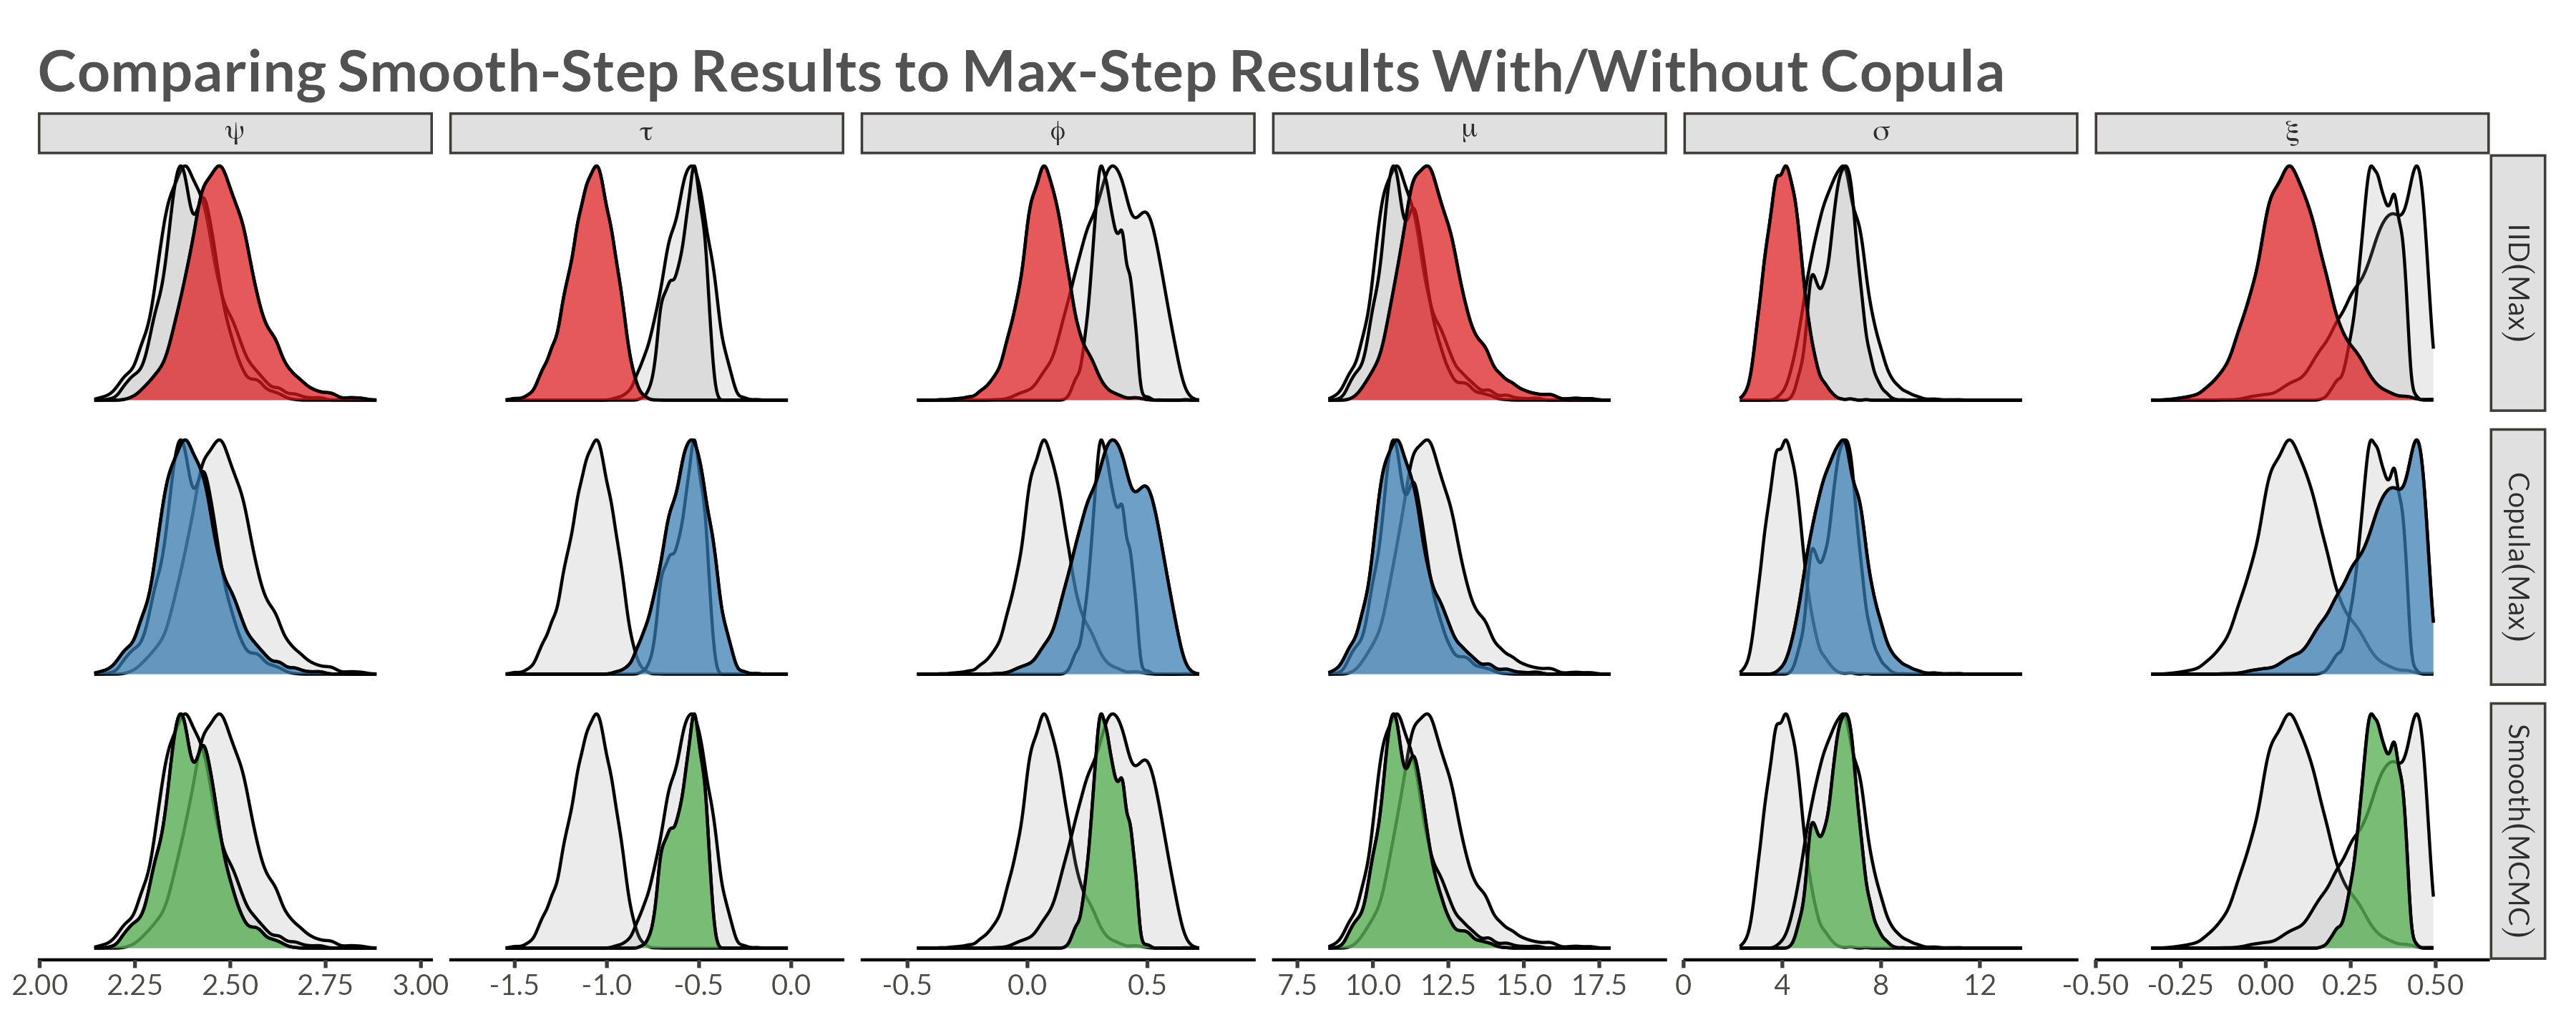
\includegraphics[width=0.8\textwidth]{Figures/max_smooth_compare_densities.png}
    \caption{Comparison of densities from different Max-and-Smooth approaches}
    \label{fig:max_smooth_densities}
\end{figure}

\begin{figure}[!htbp]
    \centering
    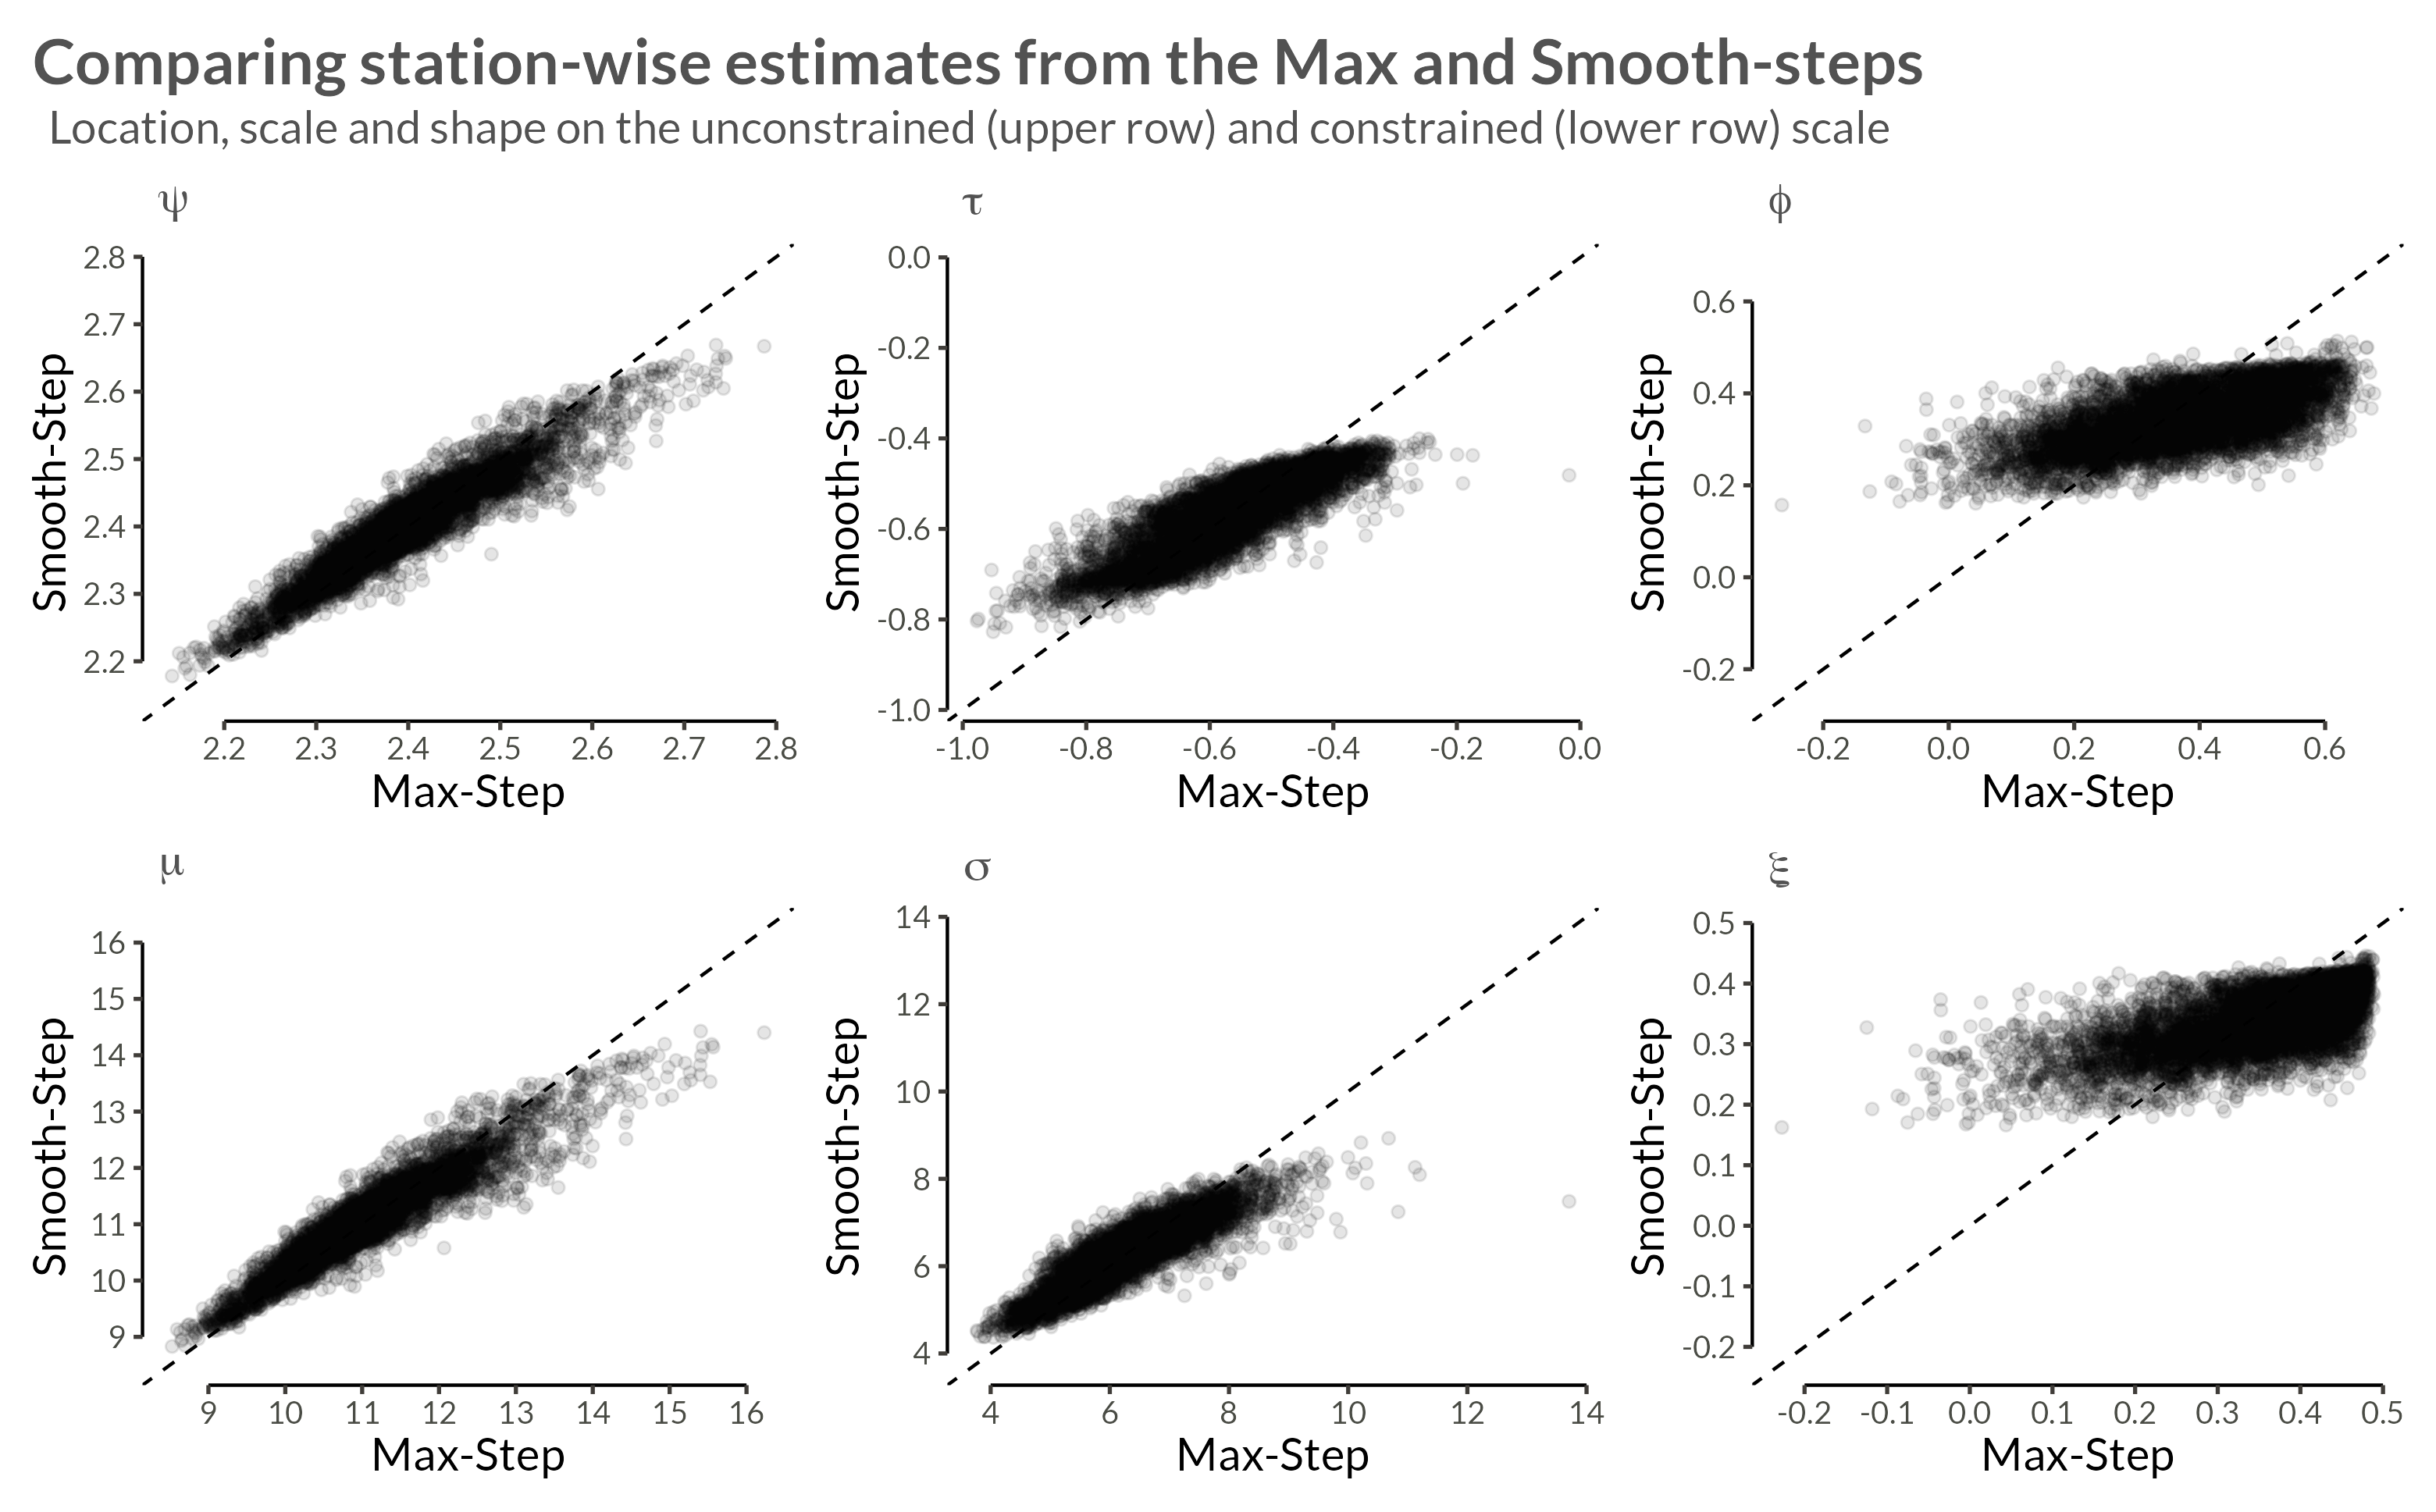
\includegraphics[width=0.8\textwidth]{Figures/max_smooth_compare_station_scatterplot.png}
    \caption{Station comparison scatterplot for Max-and-Smooth methods}
    \label{fig:max_smooth_scatterplot}
\end{figure}

\clearpage
\subsection{Spatial Analysis}

\subsubsection{Location Parameter}

\begin{figure}[!htbp]
    \centering
    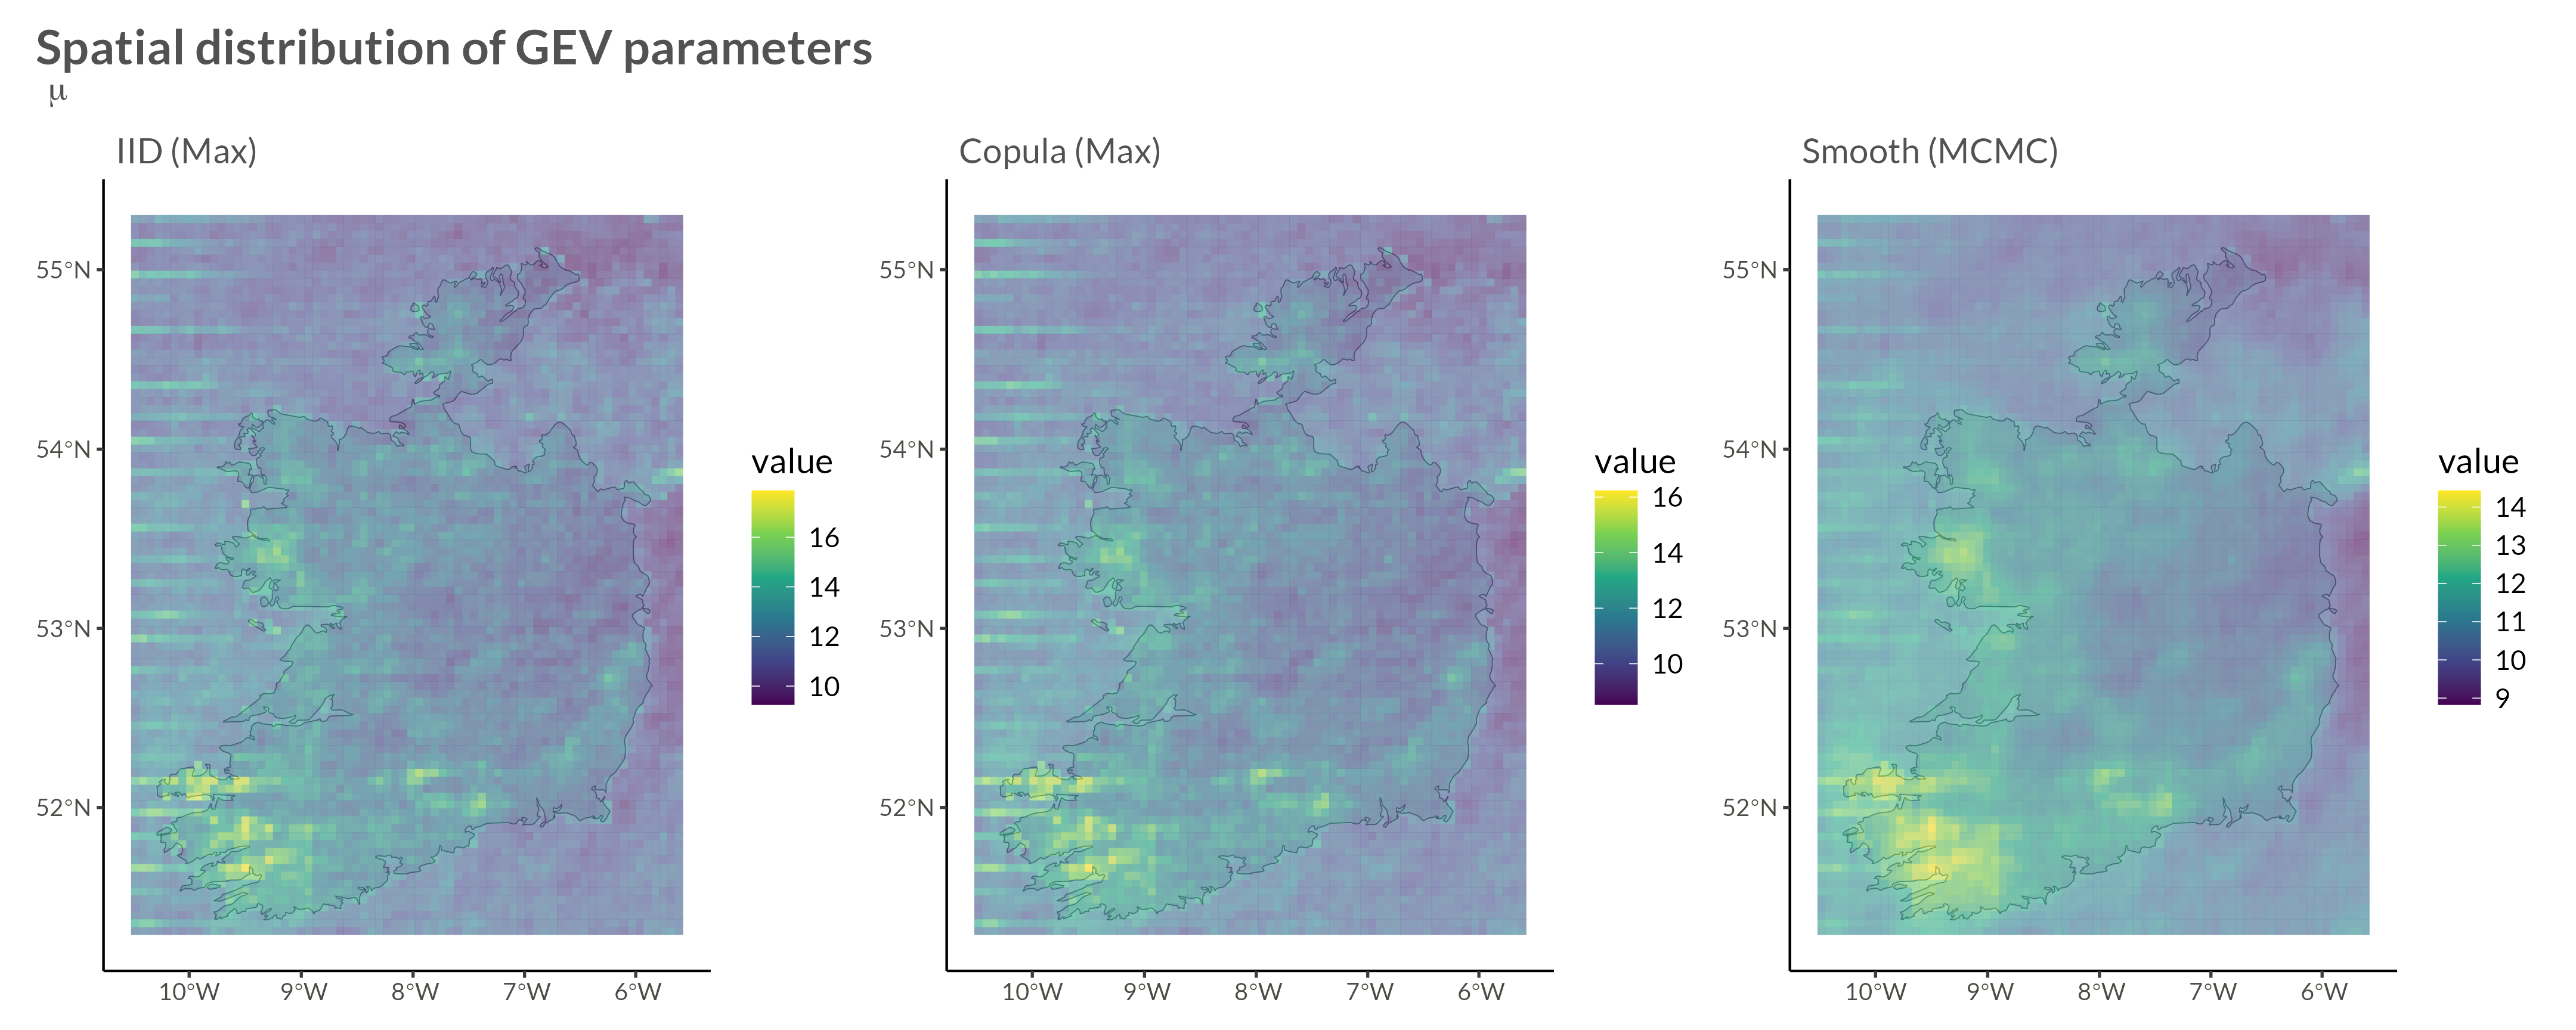
\includegraphics[width=0.75\textwidth]{Figures/location_constrained_spatial.png}
    \caption{Spatial distribution of location parameter (constrained)}
    \label{fig:location_constrained}
\end{figure}

\begin{figure}[!htbp]
    \centering
    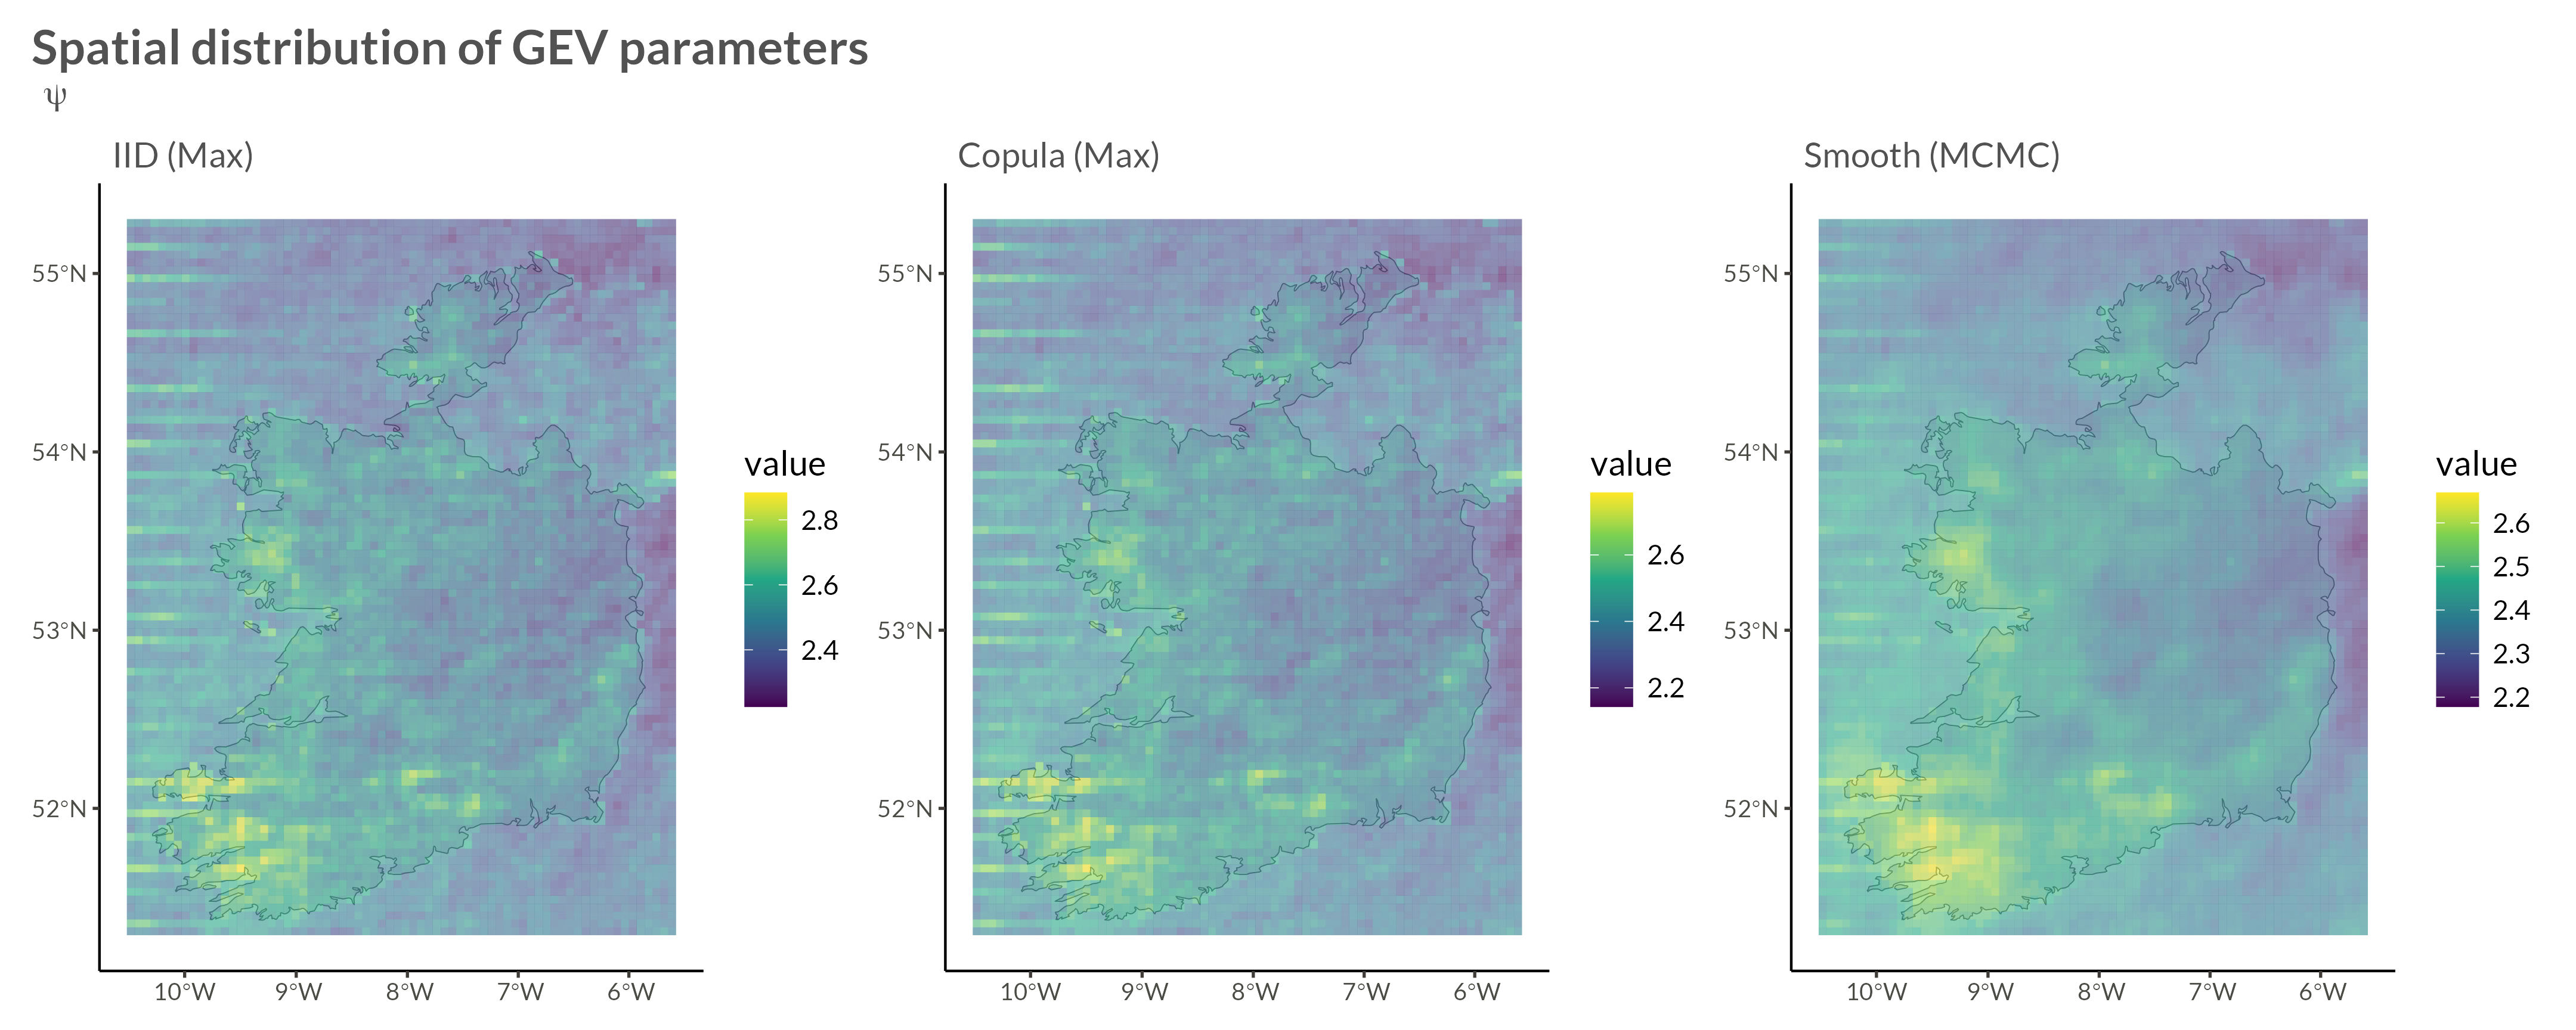
\includegraphics[width=0.75\textwidth]{Figures/location_unconstrained_spatial.png}
    \caption{Spatial distribution of location parameter (unconstrained)}
    \label{fig:location_unconstrained}
\end{figure}

\clearpage
\subsubsection{Scale Parameter}

\begin{figure}[!htbp]
    \centering
    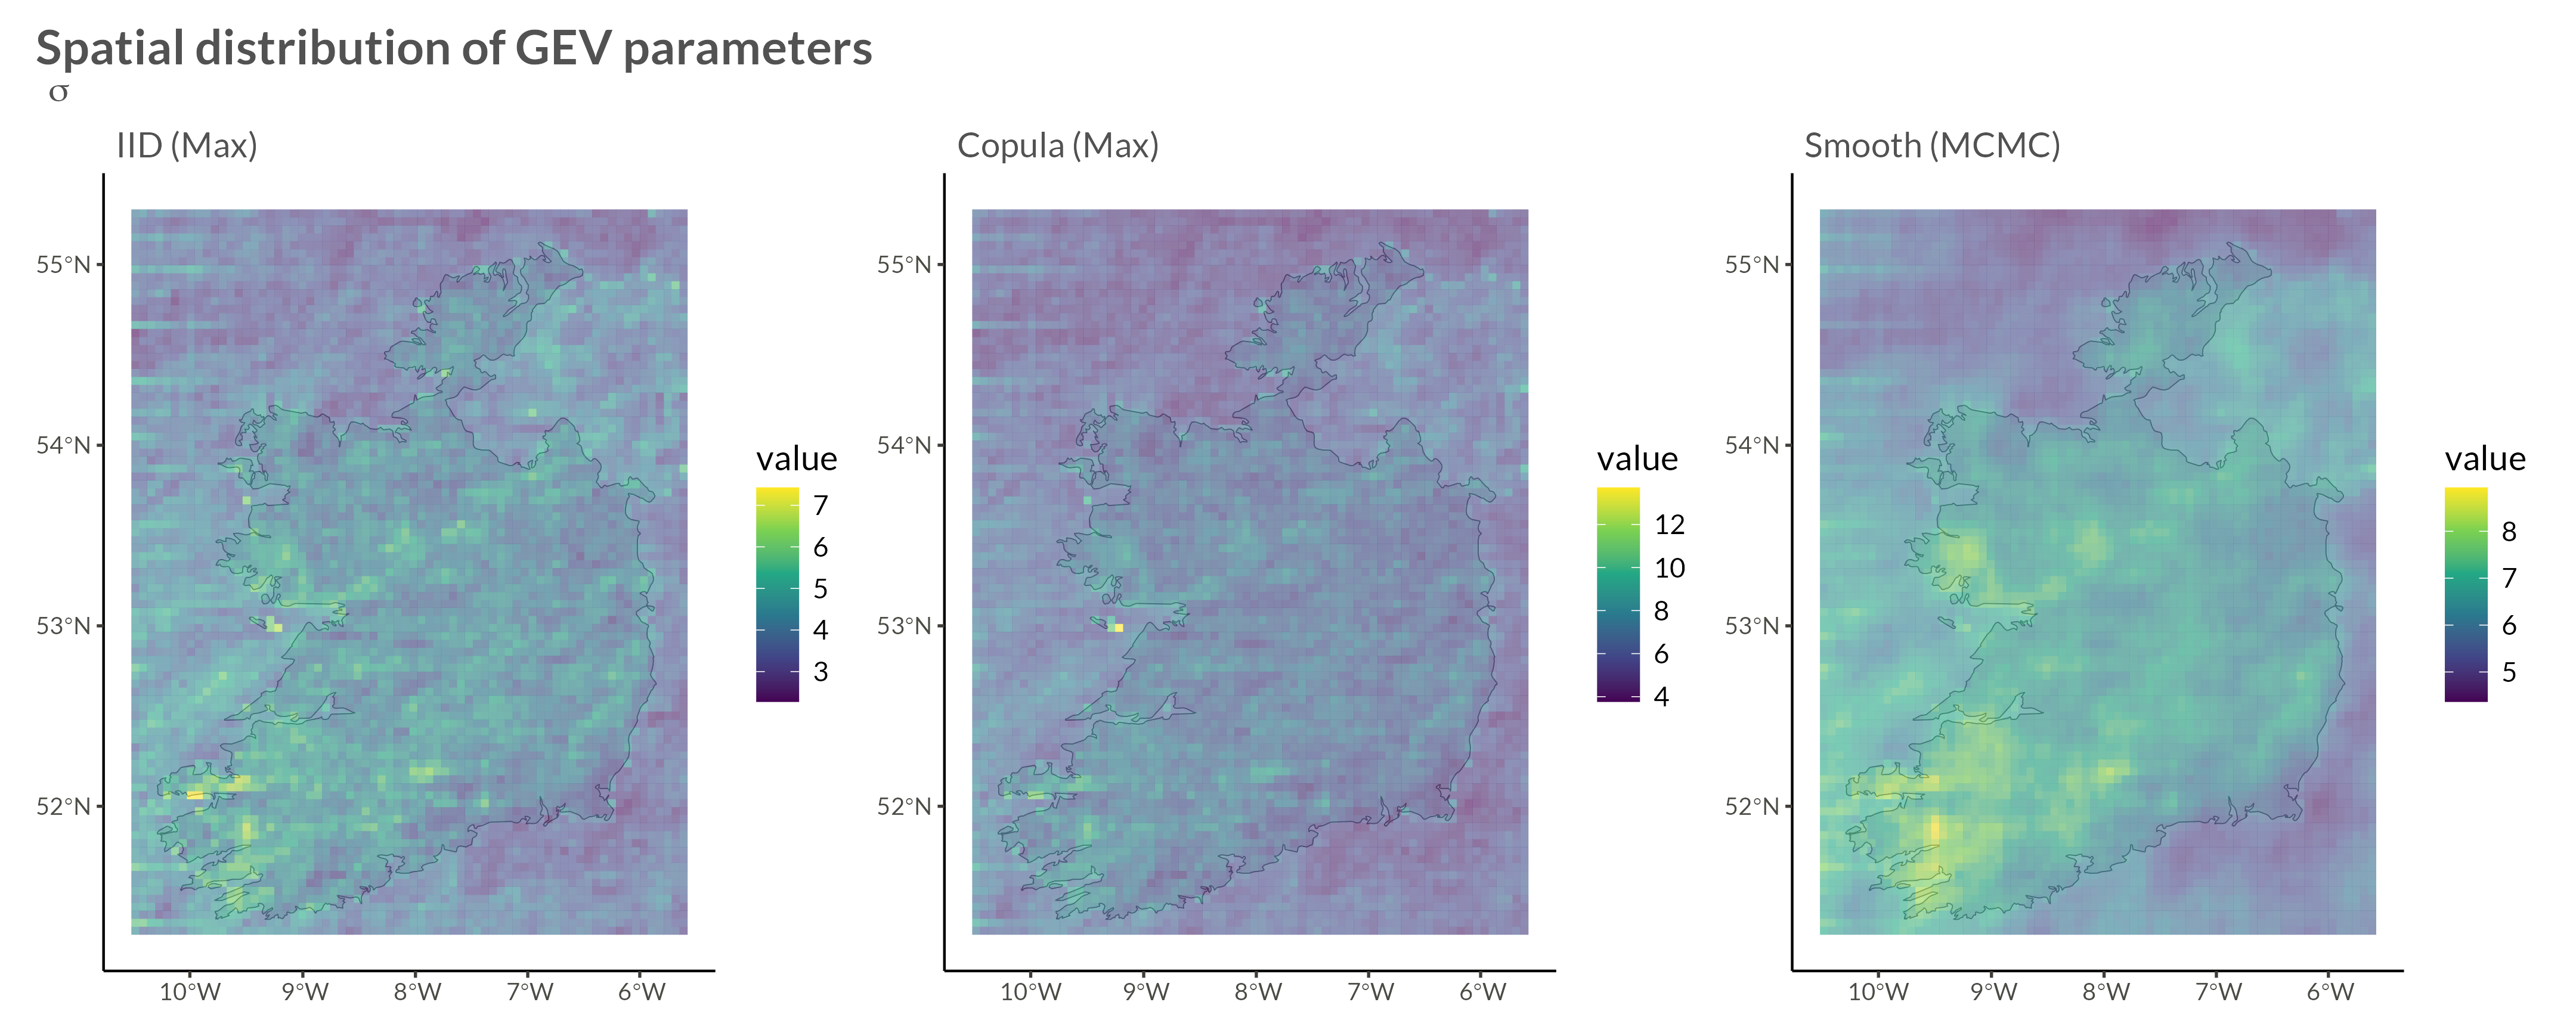
\includegraphics[width=0.75\textwidth]{Figures/scale_constrained_spatial.png}
    \caption{Spatial distribution of scale parameter (constrained)}
    \label{fig:scale_constrained}
\end{figure}

\begin{figure}[!htbp]
    \centering
    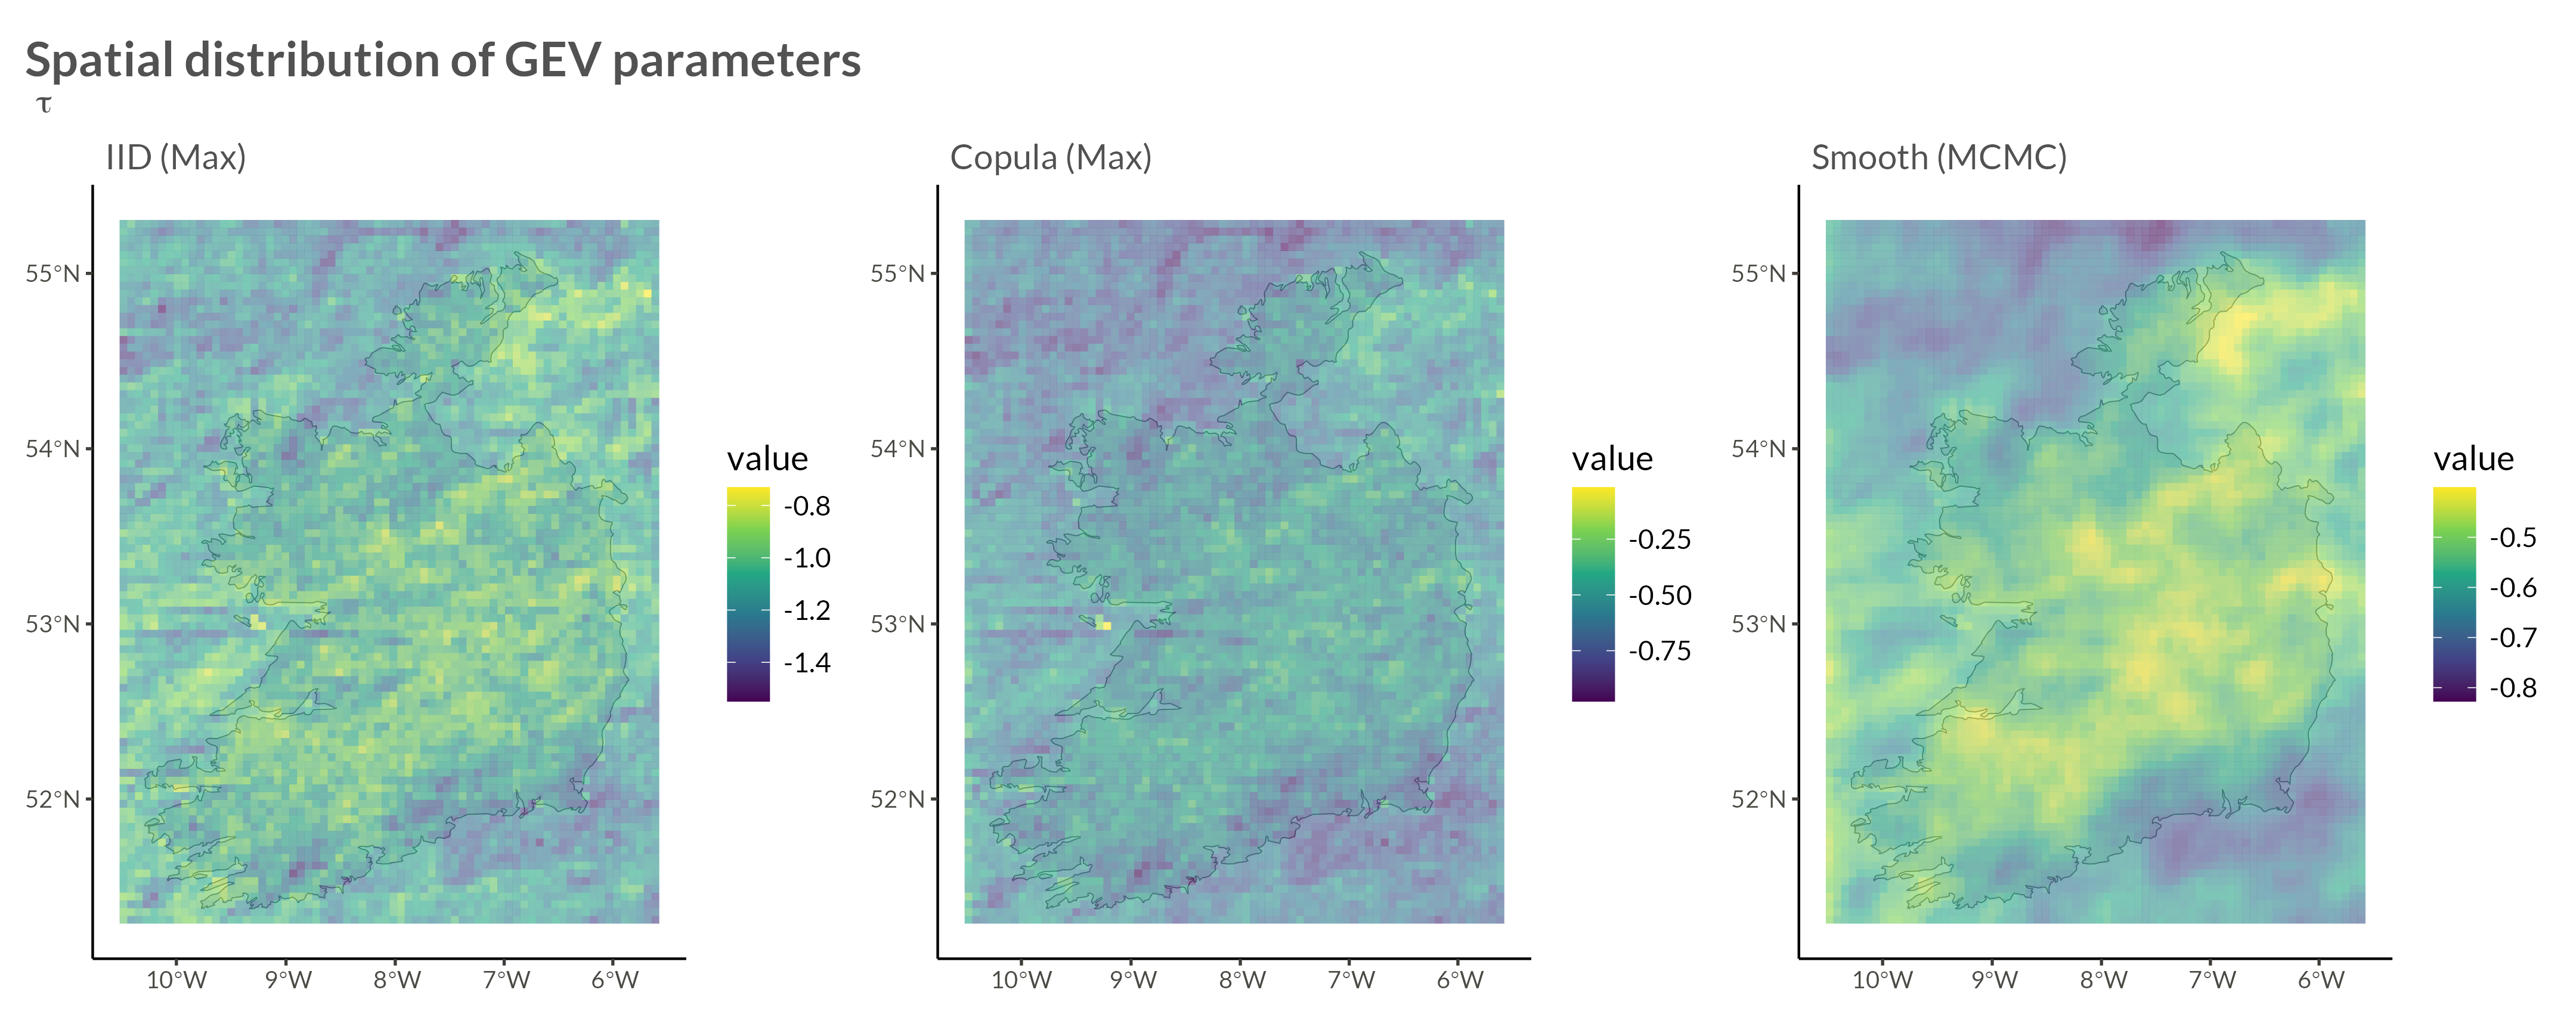
\includegraphics[width=0.75\textwidth]{Figures/scale_unconstrained_spatial.png}
    \caption{Spatial distribution of scale parameter (unconstrained)}
    \label{fig:scale_unconstrained}
\end{figure}

\clearpage
\subsubsection{Shape Parameter}

\begin{figure}[!htbp]
    \centering
    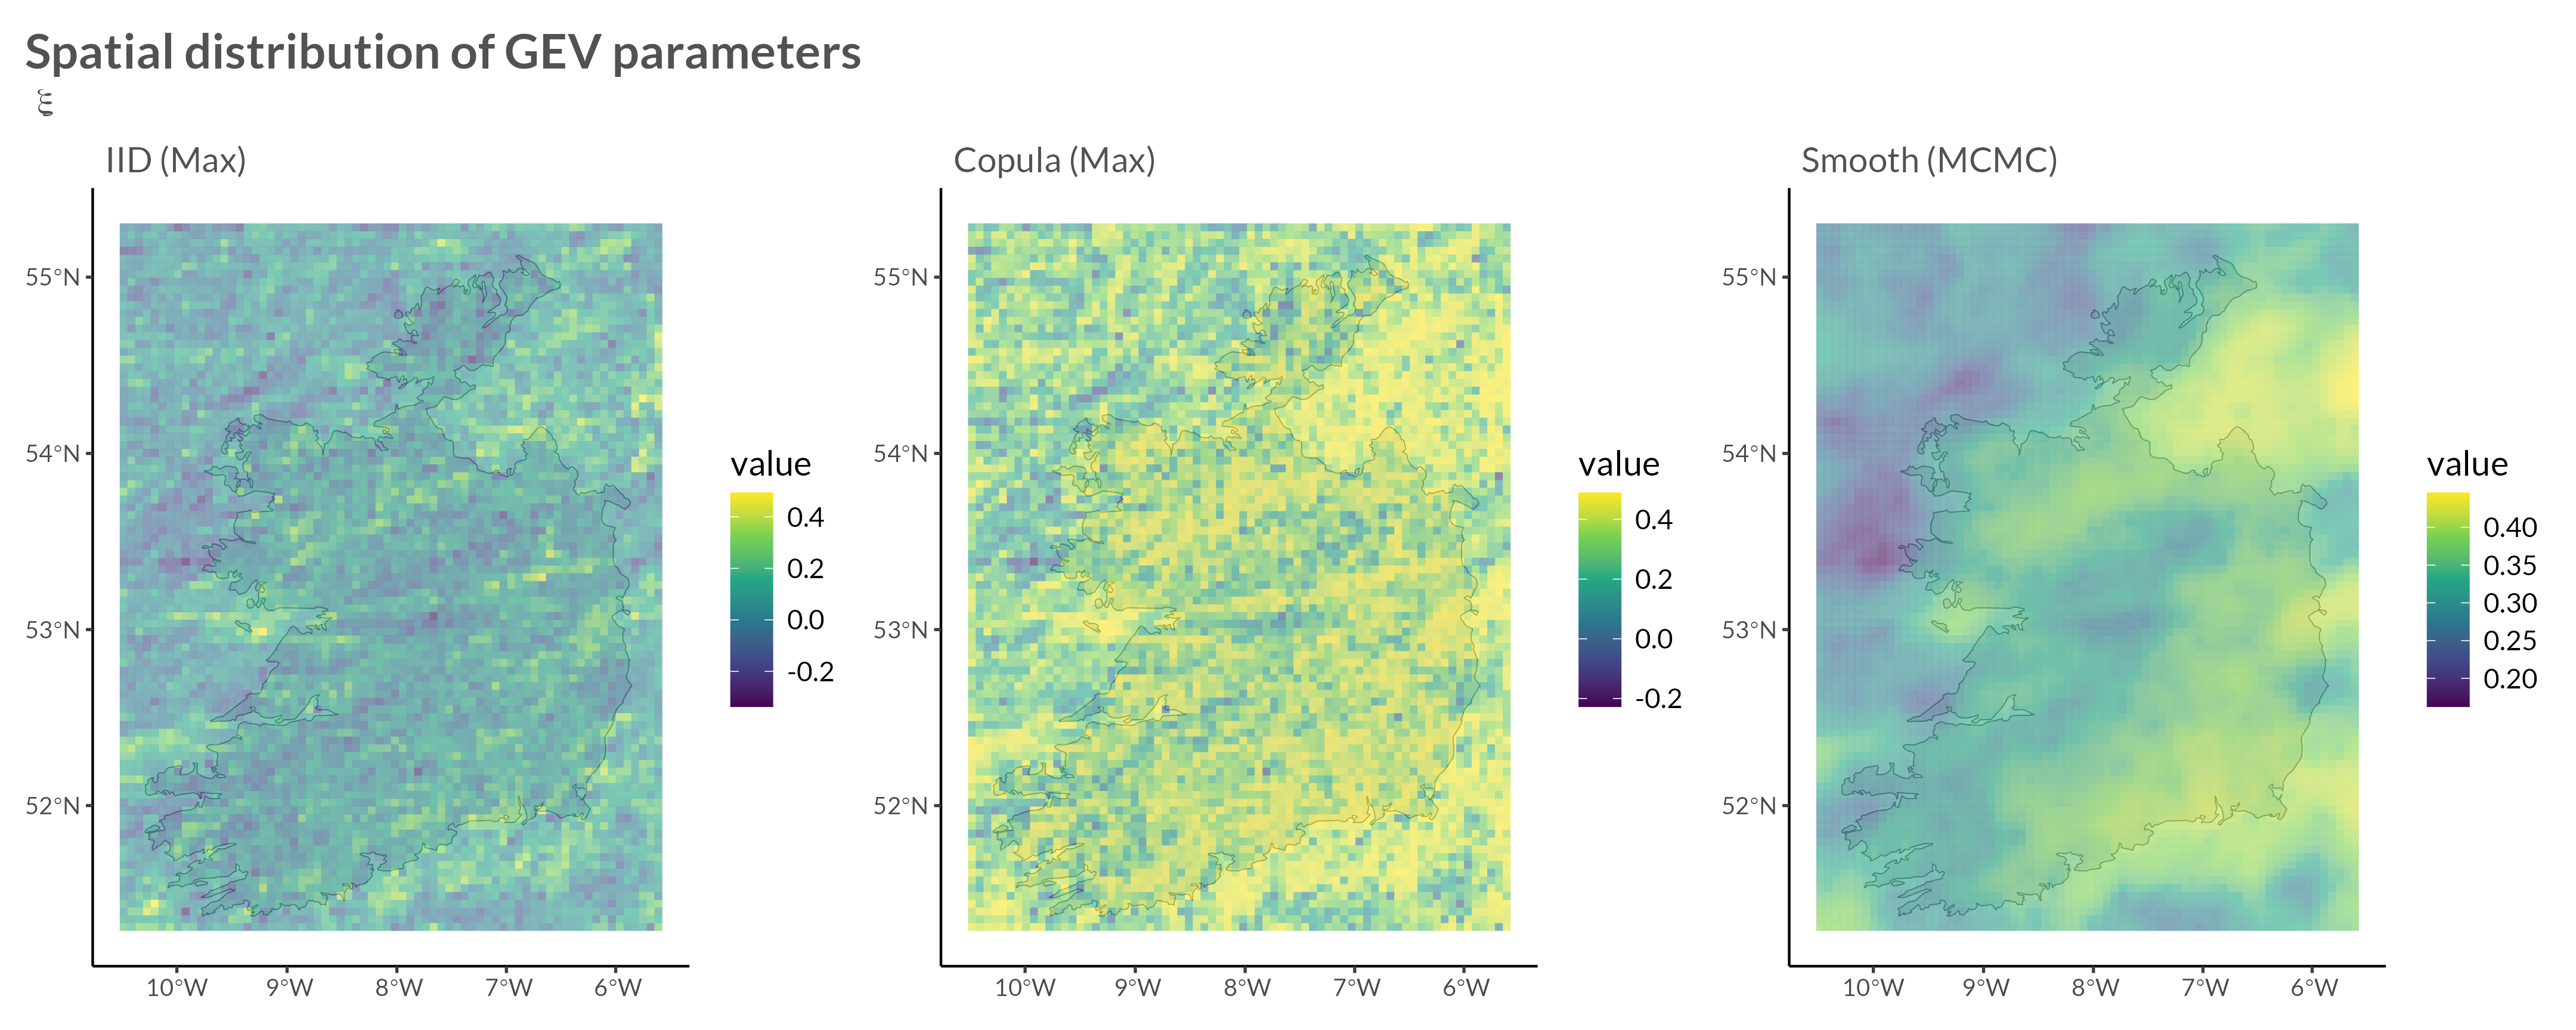
\includegraphics[width=0.75\textwidth]{Figures/shape_constrained_spatial.png}
    \caption{Spatial distribution of shape parameter (constrained)}
    \label{fig:shape_constrained}
\end{figure}

\begin{figure}[!htbp]
    \centering
    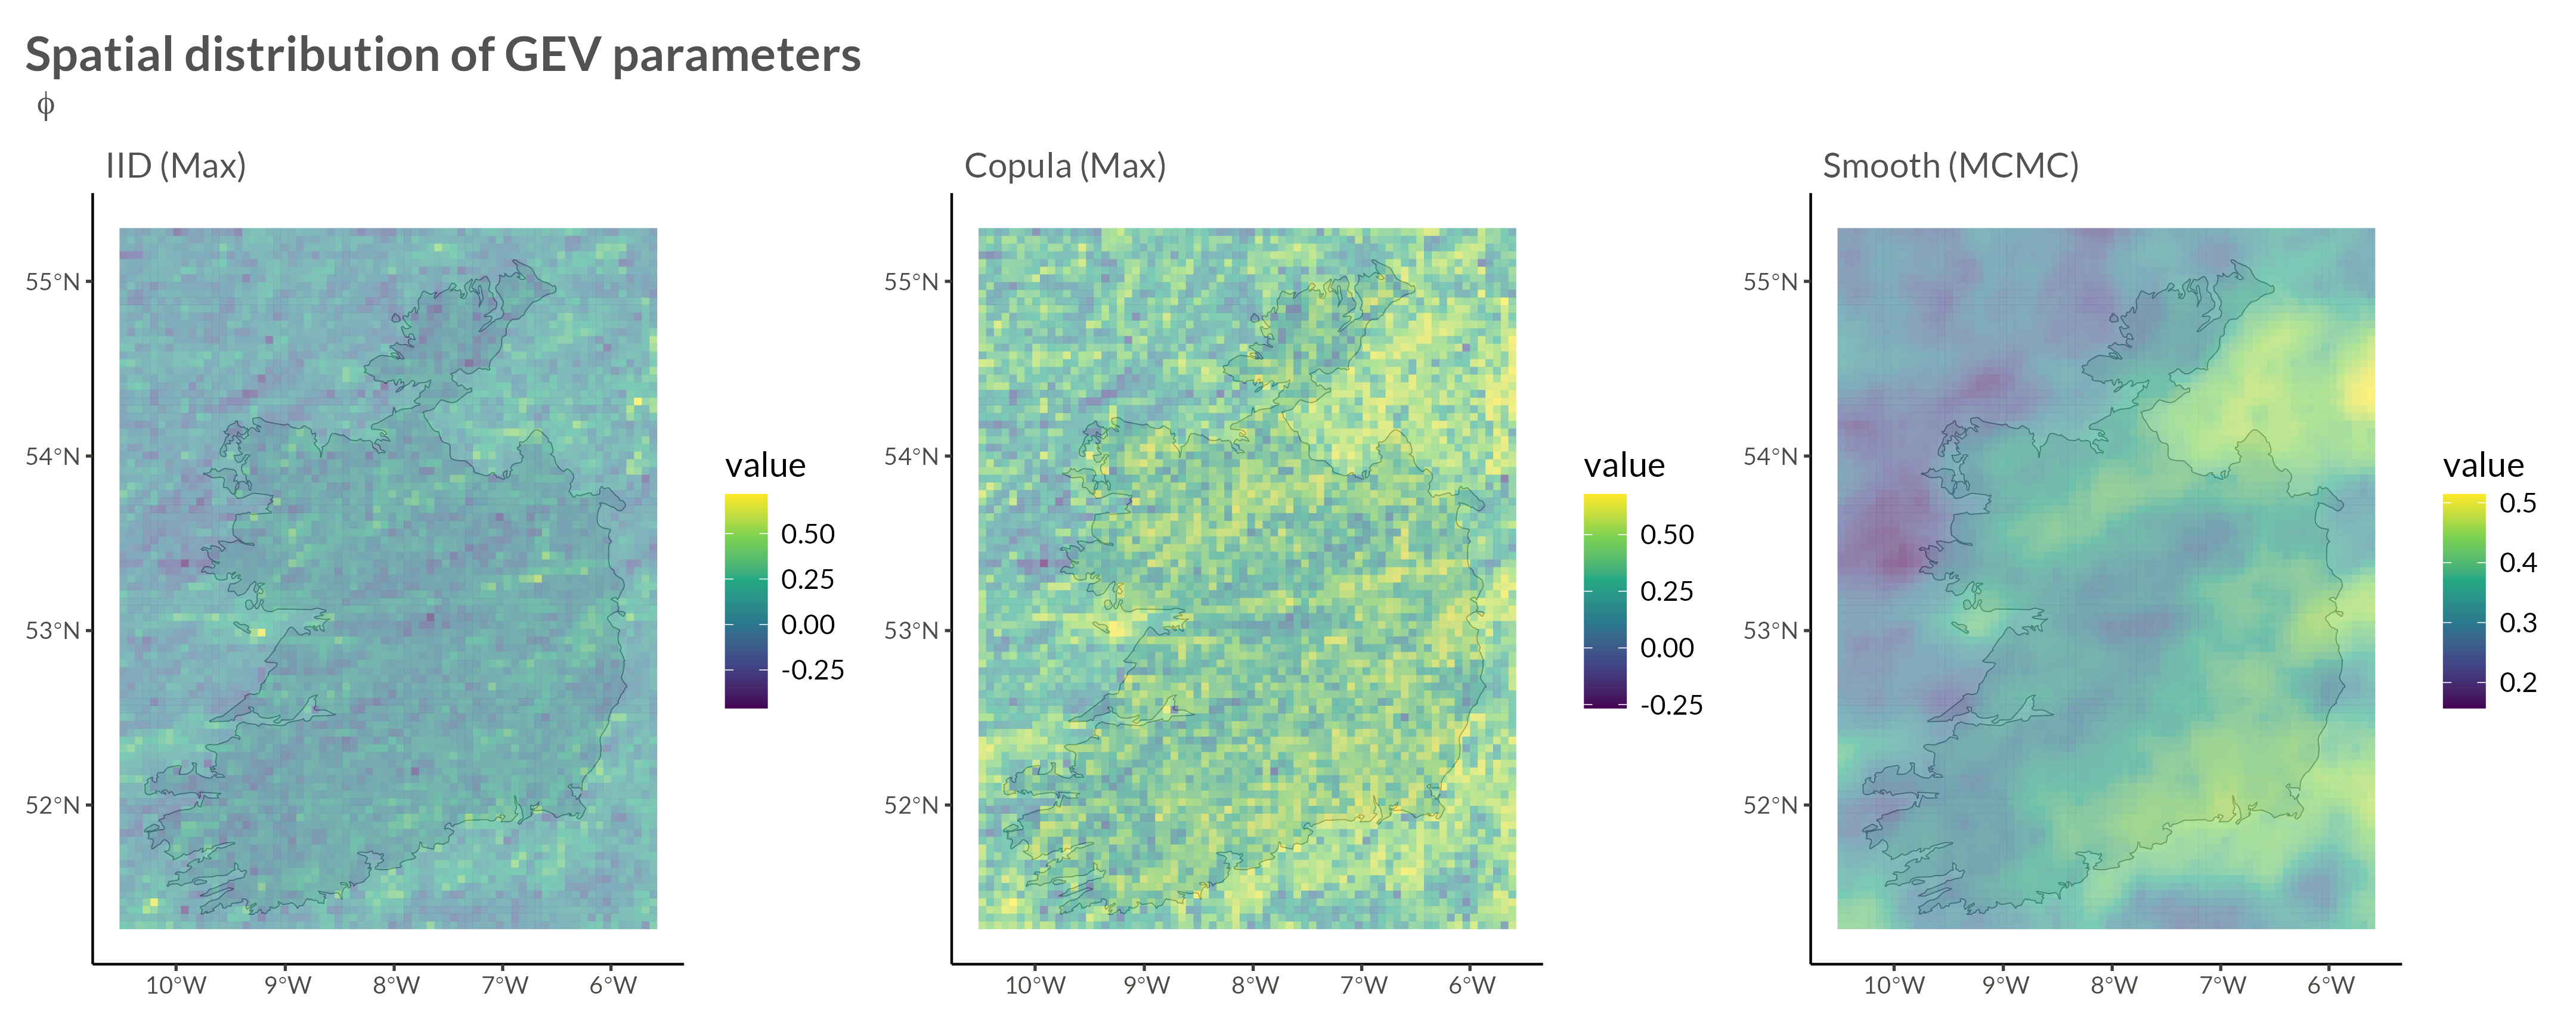
\includegraphics[width=0.75\textwidth]{Figures/shape_unconstrained_spatial.png}
    \caption{Spatial distribution of shape parameter (unconstrained)}
    \label{fig:shape_unconstrained}
\end{figure} 

\section{Conclusions}
\label{sec:conclusion}
% Chapter 7: Conclusions 


\bibliographystyle{plainnat}
\bibliography{bibliography}

\end{document} 